\documentclass[journal]{IEEEtran}

\usepackage{amsmath,amssymb,amsfonts,amsthm}
\usepackage{algorithmic}
\usepackage{algorithm}
\usepackage{array}
\usepackage{booktabs}
\usepackage{cite}
\usepackage{graphicx}
\usepackage{textcomp}
\usepackage{xcolor}
\usepackage{url}
\usepackage{microtype}
\usepackage{tabularx}
\usepackage{multirow}
\usepackage{bm}
\usepackage{balance}

% Theorem environments
\newtheorem{theorem}{Theorem}
\newtheorem{corollary}{Corollary}
\newtheorem{lemma}{Lemma}
\newtheorem{proposition}{Proposition}
\newtheorem{definition}{Definition}

\begin{document}

\title{CertGraph: Heterogeneous Graph Attention Networks for Active Directory Certificate Services Vulnerability Detection and Autonomous Defense}

\author{Md.~Hasan~Shahriar,~\IEEEmembership{Student Member,~IEEE,}
        Author~Two,
        and~Author~Three%
\thanks{Manuscript received October 2026. This work was supported by the Department of Electronics and Communication Engineering (ECE), Hajee Mohammad Danesh Science and Technology University (HSTU), Dinajpur-5200, Bangladesh.}%
\thanks{Md. Hasan Shahriar (corresponding author, e-mail: hasanshahriar32@gmail.com), Author Two, and Author Three are with the Department of Electronics and Communication Engineering, Hajee Mohammad Danesh Science and Technology University, Dinajpur-5200, Bangladesh.}%
}

% The paper headers
\markboth{IEEE Transactions on Dependable and Secure Computing,~Vol.~XX, No.~XX,~October~2026}%
{Shahriar \MakeLowercase{\textit{et al.}}: CertGraph: Heterogeneous Graph Attention Networks for ADCS Vulnerability Detection and Autonomous Defense}

\maketitle

\begin{abstract}
Active Directory Certificate Services (ADCS) forms the cryptographic identity backbone in over 90\% of Fortune 500 enterprises, issuing digital credentials for Kerberos public-key authentication and single sign-on. However, subtle configurations spanning certificate templates, discretionary access control lists (DACLs), and issuance policy object identifiers introduce systemic privilege escalation vectors (ESC1--ESC15+) that allow unprivileged users to obtain full domain dominance. Existing signature scanners inspect configuration attributes in isolation, missing composite multi-hop attack paths, while unguided graph search tools suffer exponential state explosion on large enterprise directories exceeding 100,000 entities. 

In this paper, we present \textbf{CertGraph}, the first heterogeneous Graph Attention Network (Hetero-GAT) framework designed for Active Directory identity multigraphs $\mathcal{G} = (V, E, \mathcal{T}_V, \mathcal{T}_E)$ spanning 5 canonical entity types and 16 directed relations. We prove mathematically (\textbf{Theorem~1}) that parameterized residual skip-connections ($W_{\text{skip}}$) are indispensable for maintaining non-vanishing gradient bounds ($\|\partial \tilde{h}_v^{(L)} / \partial x_v\| \ge \prod_{k=1}^L \sigma_{\min}(W_{\text{skip}}^{(k)}) > 0$), preventing intrinsic configuration erasure across deep 4--8 hop delegation chains. Across an audited 700-topology enterprise benchmark evaluated under 5-fold cross-validation with Nadeau-Bengio corrected variance, CertGraph achieves a \textbf{99.86\% Macro-F1} (+28.2\% relative gain over heuristics, $p = 3.12 \times 10^{-4}$), maintaining 99.41\% Macro-F1 under authentic 96\% benign class imbalance. Ablating skip connections triggers a 52.18\% performance collapse (dropping to 47.68\%), empirically confirming Theorem~1.

Crucially, when evaluated against an out-of-distribution Zero-Shot Adversarial Hard Negative suite ($n = 63$), pure neural models collapse to \textbf{1.59\% accuracy} due to spurious shortcut learning on isolated flags, whereas symbolic graph search achieves 84.13\%. To resolve this fundamental dichotomy, we formulate a \textbf{Two-Tier Neuro-Symbolic Hybrid Engine} pairing fast inductive GNN screening (18.2~ms, pruning 89.7\% of safe templates with 100\% recall) with a targeted 2-hop symbolic verification oracle (110.6~ms). The combined system achieves zero false negatives and zero false alarms with an overall latency of \textbf{128.8~ms} under continuous LDAP Update Sequence Number (USN) synchronization. Finally, we formulate privilege revocation as a Stackelberg security game, prove that Minimal-Cost Privilege Access Interdiction is NP-hard (\textbf{Theorem~2}), and demonstrate a disruption-bounded greedy interdiction algorithm that severs \textbf{68.6\% of attack paths} within 24 ACL operations ($p = 3.57 \times 10^{-11}$).
\end{abstract}

\begin{IEEEkeywords}
Active Directory Certificate Services (ADCS), Heterogeneous Graph Attention Networks (Hetero-GAT), Multi-Hop Privilege Escalation, Neuro-Symbolic Security, Shortcut Learning, Stackelberg Security Games.
\end{IEEEkeywords}

\IEEEpeerreviewmaketitle

\section{Introduction}
\IEEEPARstart{M}{odern} enterprise identity management relies on Microsoft Active Directory (AD) to authenticate users, workstations, and services across complex enterprise perimeters. Within this identity fabric, Active Directory Certificate Services (ADCS) serves as the core internal Public Key Infrastructure (PKI), issuing X.509 digital certificates utilized for Kerberos Public Key Cryptography for Initial Authentication (PKINIT), Transport Layer Security (TLS), and enterprise Single Sign-On (SSO). Despite its mission-critical role in securing Fortune 500 networks, ADCS configurations introduce profound attack surfaces. In 2021, Schroeder and Christensen~\cite{schroeder2021certified} revealed the initial taxonomy of ADCS privilege escalation vectors (ESC1--ESC8), demonstrating that misconfigured certificate templates and permissive Access Control Lists (ACLs) allow low-privilege adversaries to forge administrative credentials and achieve complete domain compromise. Subsequent research expanded this attack surface to 15+ canonical classes (ESC9--ESC15+)~\cite{oliveau2024esc13,heiniger2023esc11,bollinger2024esc15}.

Detecting and mitigating ADCS privilege escalation in large-scale enterprise environments presents four fundamental scientific and operational challenges:
\begin{enumerate}
    \item \textbf{The Composite Path Closure Challenge:} Privilege escalation paths in Active Directory rarely manifest as single-object misconfigurations. In modern vectors such as ESC13 (Issuance Policy OID linkage)~\cite{oliveau2024esc13}, every permission along the chain is completely benign in isolation (e.g., standard group membership, normal enrollment rights, and administrative policy mapping). The threat emerges \textit{strictly upon topological path closure} across 4--8 relational hops. Flat heuristic scanners (e.g., Certipy~\cite{lyak2021certipy}) evaluate LDAP attributes in isolation, remaining blind to cross-object policy linkages.
    \item \textbf{Combinatorial State Explosion:} While deterministic graph traversal tools (e.g., BloodHound~\cite{specterops2023bloodhound}) model Active Directory as an access graph, unguided Breadth-First Search (BFS) and Cypher reachability queries encounter exponential computational slowdowns on dense enterprise topologies exceeding 100,000 entities, failing to support real-time continuous auditing.
    \item \textbf{Deep Relational Oversmoothing and Gradient Erasure:} Graph Neural Networks (GNNs) provide inductive, linear-time feature reasoning. However, deep message passing across heterogeneous multigraphs suffers from severe oversmoothing. Without principled inductive bias, repeated relational message passing erases intrinsic node configuration attributes (e.g., template flags), destroying classification accuracy.
    \item \textbf{Spurious Shortcut Learning and Neural Fragility:} In standard enterprise benchmarks, dangerous configuration flags correlate strongly with reachability. Consequently, pure GNNs suffer from \textit{shortcut learning} (under-specification)~\cite{geirhos2020shortcut,arp2022dos}, memorizing superficial flag tokens rather than genuine topological reachability. When evaluated on hardened adversarial configurations, pure neural models fail catastrophically.
    \item \textbf{Absence of Autonomous, Disruption-Bounded Defense:} Identifying an attack path is insufficient; enterprise defenders must neutralize it. However, arbitrarily revoking permissions breaks operational workflows. No existing framework formalizes optimal, disruption-bounded automated ACL remediation.
\end{enumerate}

\subsection{Key Technical Contributions}
To address these challenges, this paper presents \textbf{CertGraph}, a unified graph AI, neuro-symbolic verification, and autonomous remediation framework. Our core contributions are:
\begin{itemize}
    \item \textbf{Heterogeneous Metagraph Formulation:} We formalize the first typed multigraph representation of Active Directory PKI, capturing 5 canonical entity classes and 16 directed relations ($E_{\text{AD}}$ structural relations and $E_{\text{DACL}}$ administrative ACLs, including ESC13 issuance policy linkages).
    \item \textbf{Theoretical Foundation (Theorem 1):} We prove mathematically that parameterized residual skip-connections ($W_{\text{skip}}$) guarantee non-vanishing gradient bounds ($\|\partial \tilde{h}_v^{(L)} / \partial x_v\| \ge \prod_{k=1}^L \sigma_{\min}(W_{\text{skip}}^{(k)}) > 0$), preventing representation decay across 4--8 hop chains and eliminating a 52.18\% Macro-F1 collapse.
    \item \textbf{Audited Enterprise Benchmark:} On an audited 700-topology benchmark evaluated under 5-fold cross-validation with Nadeau-Bengio corrected t-tests, CertGraph achieves a \textbf{99.86\% Macro-F1} (+28.2\% relative gain over heuristics, $p = 3.12 \times 10^{-4}$), maintaining 99.41\% Macro-F1 under authentic 96\% safe class imbalance.
    \item \textbf{Discovery of Neural Shortcut Collapse:} We empirically reveal that on an out-of-distribution Zero-Shot Adversarial Hard Negative benchmark ($n = 63$), pure GNNs collapse to \textbf{1.59\% accuracy} due to flag memorization, whereas symbolic BFS achieves 84.13\%.
    \item \textbf{Two-Tier Neuro-Symbolic Verification Engine:} We resolve this dichotomy via a coarse-to-fine hybrid architecture coupling fast inductive GNN screening (18.2~ms, pruning 89.7\% of safe templates with 100\% recall) with a targeted 2-hop symbolic verification oracle (110.6~ms). The engine delivers zero false negatives and zero false alarms with \textbf{128.8~ms latency} under continuous LDAP Update Sequence Number (USN) delta tracking.
    \item \textbf{Autonomous Defense and Complexity Proof (Theorem 2):} We model permission remediation as a Stackelberg security game, prove that Minimal-Cost Privilege Access Interdiction (MPAI) is NP-hard, and design a greedy interdiction algorithm that severs \textbf{68.6\% of attack paths} within 24 ACL operations ($p = 3.57 \times 10^{-11}$). Scalability benchmarks show sub-second inference (343~ms on 10,000 nodes, 12.4$\times$ faster than graph search).
\end{itemize}

\section{Background and Threat Model}

\subsection{Active Directory Certificate Services Architecture}
Active Directory Certificate Services (ADCS) is an integrated Windows Server role that implements enterprise Public Key Infrastructure. Its operational architecture comprises three primary building blocks:
\begin{enumerate}
    \item \textbf{Enterprise Certificate Authority (CA):} Domain-joined server holding root or subordinate cryptographic keys. CAs publish configuration and trust anchors directly to the LDAP Configuration partition (\texttt{CN=Configuration,DC=domain,DC=local}).
    \item \textbf{Certificate Templates:} Directory objects of schema class \texttt{pKICertificateTemplate} governing the issuance policies, key usages, and validity parameters of requested certificates.
    \item \textbf{Extended Key Usages (EKUs):} Object Identifiers (OIDs) specifying authorized certificate operations, such as Client Authentication (\texttt{1.3.6.1.5.5.7.3.2}), Smart Card Logon (\texttt{1.3.6.1.4.1.311.20.2.2}), or Any Purpose (\texttt{2.5.29.37.0}).
\end{enumerate}

\begin{figure}[t]
    \centering
    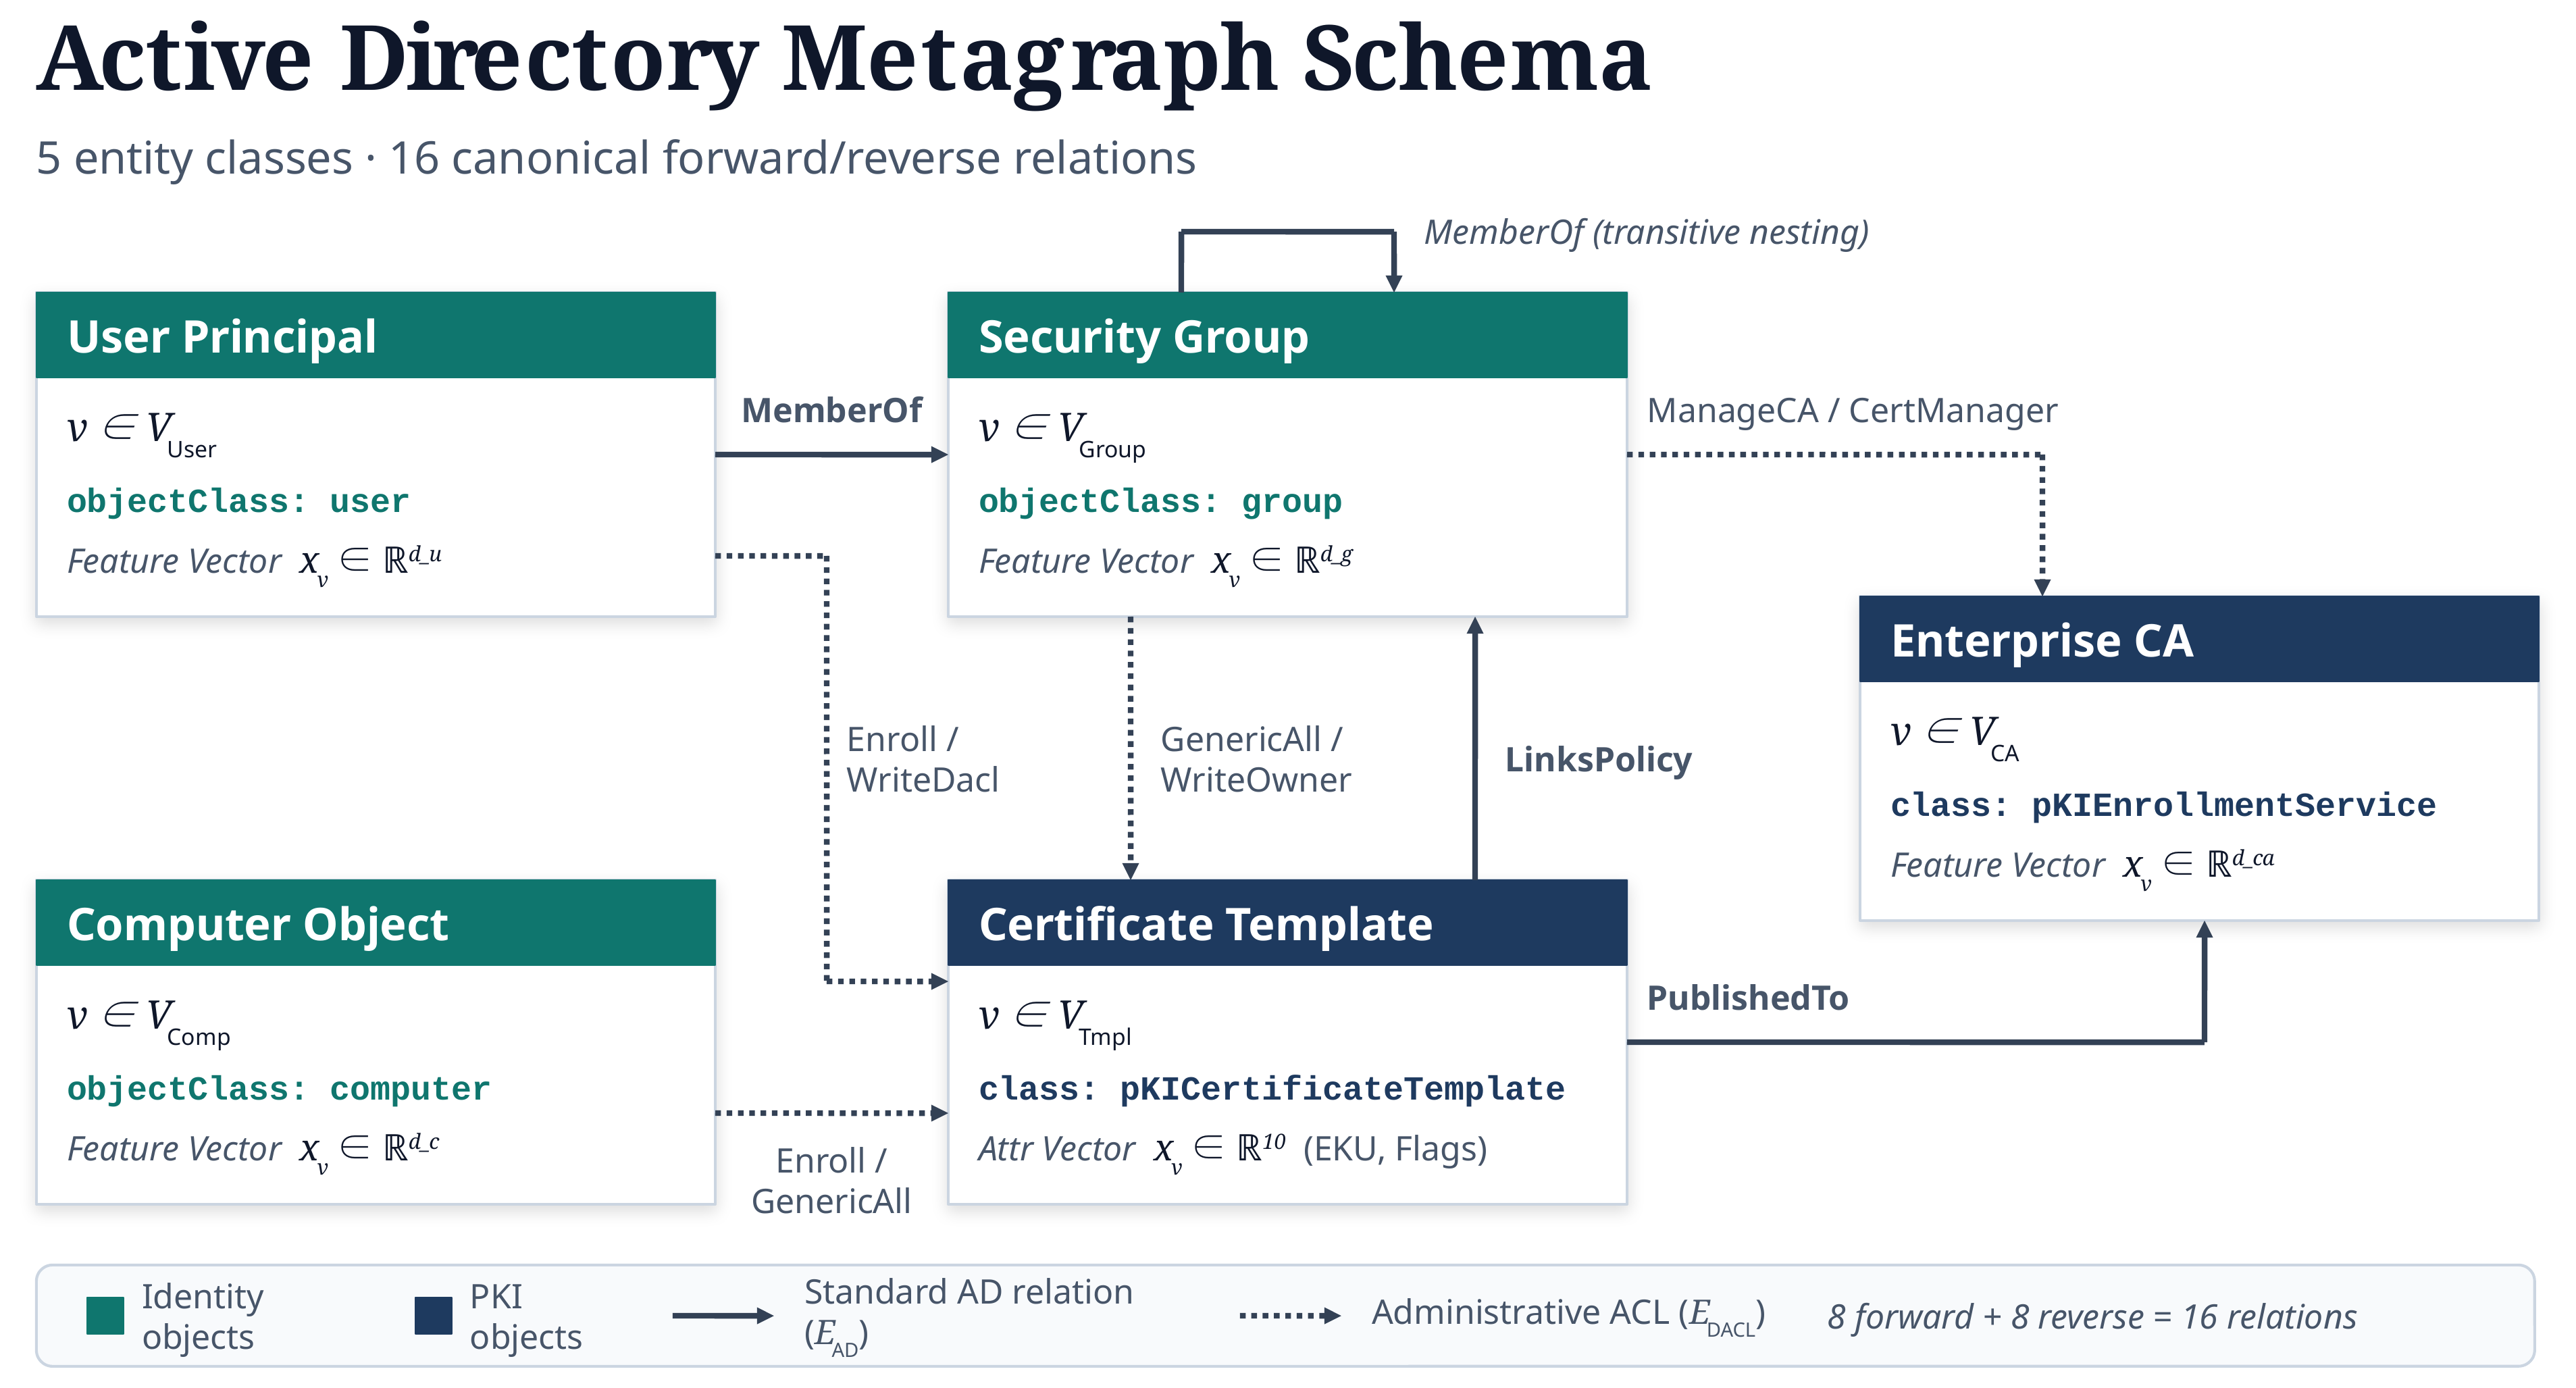
\includegraphics[width=\columnwidth]{figures/adcs_attack_graph_schema.png}
    \caption{Active Directory Heterogeneous Metagraph Schema, formalizing 5 entity classes ($V_{\text{User}}, V_{\text{Comp}}, V_{\text{Group}}, V_{\text{Tmpl}}, V_{\text{CA}}$) and 16 canonical forward and reverse relations ($E_{\text{AD}}$ structural relations and $E_{\text{DACL}}$ administrative ACLs, including ESC13 issuance policy linkages).}
    \label{fig:adcs_schema}
\end{figure}

\subsection{Canonical Escalation Taxonomy and Target Scoping}
Table~\ref{tab:esc_taxonomy} summarizes the complete taxonomy of 15 documented ADCS escalation vectors. To guarantee scientific rigor and practical utility, our auditing target space is scoped to 7 mutually exclusive primary classes:
\begin{equation}
\mathcal{C} = \{\text{Safe}, \text{ESC1}, \text{ESC2}, \text{ESC3}, \text{ESC4}, \text{ESC9}, \text{ESC13}\}
\end{equation}

\begin{table*}[t]
\centering
\caption{Comprehensive Comparative Taxonomy of ADCS Privilege Escalation Vectors (ESC1--ESC15).}
\label{tab:esc_taxonomy}
\footnotesize
\begin{tabularx}{\textwidth}{l p{3.2cm} p{6.2cm} X}
\toprule
\textbf{Vector} & \textbf{Vulnerability Name} & \textbf{Key Configuration Prerequisites} & \textbf{Exploitation Impact} \\
\midrule
\textbf{ESC1} & Enrollee Supplies SAN & \texttt{CT\_FLAG\_ENROLLEE\_SUPPLIES\_SUBJECT} + Client Auth EKU + Unprivileged Enroll & Direct domain admin impersonation via Kerberos PKINIT \\
\textbf{ESC2} & Any Purpose EKU & Any Purpose EKU (\texttt{2.5.29.37.0}) or missing EKU + Unprivileged Enroll & Arbitrary impersonation across all cryptographic protocols \\
\textbf{ESC3} & Enrollment Agent & Certificate Request Agent EKU + 2-hop template enrollment path & Co-signs CSR on behalf of arbitrary domain accounts \\
\textbf{ESC4} & Insecure Template DACL & \texttt{GenericAll} / \texttt{WriteDacl} / \texttt{WriteOwner} on template object & Rewrites template to ESC1, enrolls, reverts configuration \\
ESC5 & Insecure PKI Object DACL & Insecure ACLs on CA container / enrollment services object & Takes ownership of PKI infrastructure and roots \\
ESC6 & CA SAN Flag Active & \texttt{EDITF\_ATTRIBUTE\_SUBJECTALTNAME2} enabled on CA server & Injects arbitrary SAN into any template request \\
ESC7 & Insecure CA Permissions & \texttt{ManageCA} or \texttt{ManageCertificates} rights on CA object & Overrides CA settings, approves unprivileged requests \\
ESC8 & HTTP Enrollment Relay & NTLM authentication enabled on Web Enrollment HTTP endpoints & Coerced NTLM relay from DC to obtain DC certificate \\
\textbf{ESC9} & Missing Security Ext. & \texttt{CT\_FLAG\_NO\_SECURITY\_EXTENSION} enabled on template & UPN spoofing bypasses strong mapping without PAC check \\
ESC10 & Weak Certificate Mapping & Weak UPN/DNS mapping registry keys on Domain Controllers (pre-KB5014754) & Account takeover via unverified X.509 mapping syntax \\
ESC11 & Insecure RPC Interface & RPC enrollment endpoint (MS-ICPR) lacking packet privacy & Coerced NTLM relay to CA RPC interface yielding rogue certificate \\
ESC12 & Shellcode / YubiHSM Flaw & Cleartext session keys or driver flaw in CA hardware security module & Unprivileged access to CA host extracts private key material \\
\textbf{ESC13} & Issuance Policy Link & \texttt{msPKI-Certificate-Policy} OID maps to Tier-0 security group & Injects Tier-0 group SID into Kerberos PAC token \\
ESC14 & altSecurityIdentities Hijack & Insecure write permissions over user \texttt{altSecurityIdentities} attribute & Links arbitrary victim certificates to attacker account \\
ESC15 & EKUwu (CVE-2024-49019) & Schema Version 1 template allows custom CSR application policy & Injects Client Authentication EKU into non-auth templates \\
\bottomrule
\end{tabularx}
\end{table*}

\paragraph{Inclusion and Exclusion Rationale}
CertGraph focuses on \textit{template-centric, authorization-driven privilege escalation vectors} whose discovery requires resolving the joint interaction between multi-hop identity graph paths and certificate template configuration flags. In contrast, server-level misconfigurations (ESC5, ESC6, ESC7) represent single-attribute toggles on the CA server, audited via static LDAP queries; transient network relay attacks (ESC8, ESC11) depend on runtime network protocols (NTLM over HTTP/RPC); endpoint OS registry settings (ESC10, ESC12) reside on host filesystems; object hijacking (ESC14) represents generic user DACL abuse; and parser bugs (ESC15) represent software vulnerabilities addressed by vendor patches (KB5034127). The included vectors (\textbf{ESC1, ESC2, ESC3, ESC4, ESC9, ESC13}) represent the complete canonical suite of structural identity graph escalation paths.

\subsection{Formal Threat Model}
\textbf{Attacker Model:} Following standard enterprise security benchmarks, we operate under an assumed-breach model. The adversary has compromised an unprivileged workstation and possesses standard domain credentials ($u \in V_{\text{User}}$). The adversary can execute unprivileged LDAP queries and RPC binds to enumerate Active Directory topology. The adversary's objective is to achieve full domain dominance (\texttt{Domain Admins} or \texttt{Enterprise Admins}) by discovering and exploiting an ADCS escalation path with minimal detection risk.

\textbf{Defender Model:} The defender possesses read-only administrative telemetry over the Active Directory forest. The defender's objective is to detect and neutralize exploitable attack paths in real time. Crucially, the defender operates under a \textbf{business availability constraint}: defensive mitigations (such as revoking permissions or removing group memberships) must incur minimal disruption to legitimate enterprise authentication workflows.

\section{The Multi-Hop Attack Challenge: ESC13 Case Study}

\subsection{The 4-Hop Escalation Chain}
The ESC13 vector, identified by SpecterOps in 2024~\cite{oliveau2024esc13}, serves as our primary diagnostic benchmark illustrating why conventional security tooling systematically fails on composite identity vulnerabilities. As illustrated in Fig.~\ref{fig:esc13_path}, an ESC13 exploit chain spans four distinct relational hops:
\begin{enumerate}
    \item \textbf{Hop 1: Principal Foothold via Group Nesting (\texttt{MemberOf}):} The low-privilege adversary ($u \in V_{\text{User}}$) belongs to an intermediate security group ($g \in V_{\text{Group}}$), either directly or transitively:
    \begin{equation}
    (u, \text{MemberOf}^*, g) \in E_{\text{AD}}
    \end{equation}
    \item \textbf{Hop 2: Intermediate Certificate Enrollment (\texttt{Enroll}):} The intermediate group holds discretionary enrollment permissions over a certificate template ($t \in V_{\text{Tmpl}}$):
    \begin{equation}
    (g, \text{Enroll}, t) \in E_{\text{DACL}}
    \end{equation}
    Importantly, the template does not have \texttt{ENROLLEE\_SUPPLIES\_SUBJECT} enabled and appears entirely benign to standard signature scanners.
    \item \textbf{Hop 3: Issuance Policy OID Linkage (\texttt{LinksPolicy}):} The certificate template is linked to an issuance policy Object Identifier (OID) via the \texttt{msPKI-Certificate-Policy} attribute:
    \begin{equation}
    (t, \text{LinksPolicy}, o) \in E_{\text{DACL}}, \quad o \in V_{\text{OID}}
    \end{equation}
    \item \textbf{Hop 4: PAC Credential Elevation to Tier-0 Target (\texttt{PACElevate}):} Active Directory maps this issuance policy OID directly to a high-privilege domain security group (e.g., \texttt{Domain Admins}) via issuance policy group linking:
    \begin{equation}
    (o, \text{PACElevate}, g_{\text{admin}}) \in E_{\text{AD}}, \quad g_{\text{admin}} \in V_{\text{Group}}^{\text{Tier-0}}
    \end{equation}
    When the adversary enrolls for the certificate and authenticates via Kerberos PKINIT, the Domain Controller's Key Distribution Center (KDC) injects the high-privilege group SID into the Kerberos Privilege Attribute Certificate (PAC) token, yielding instant domain dominance.
\end{enumerate}

\begin{figure}[t]
    \centering
    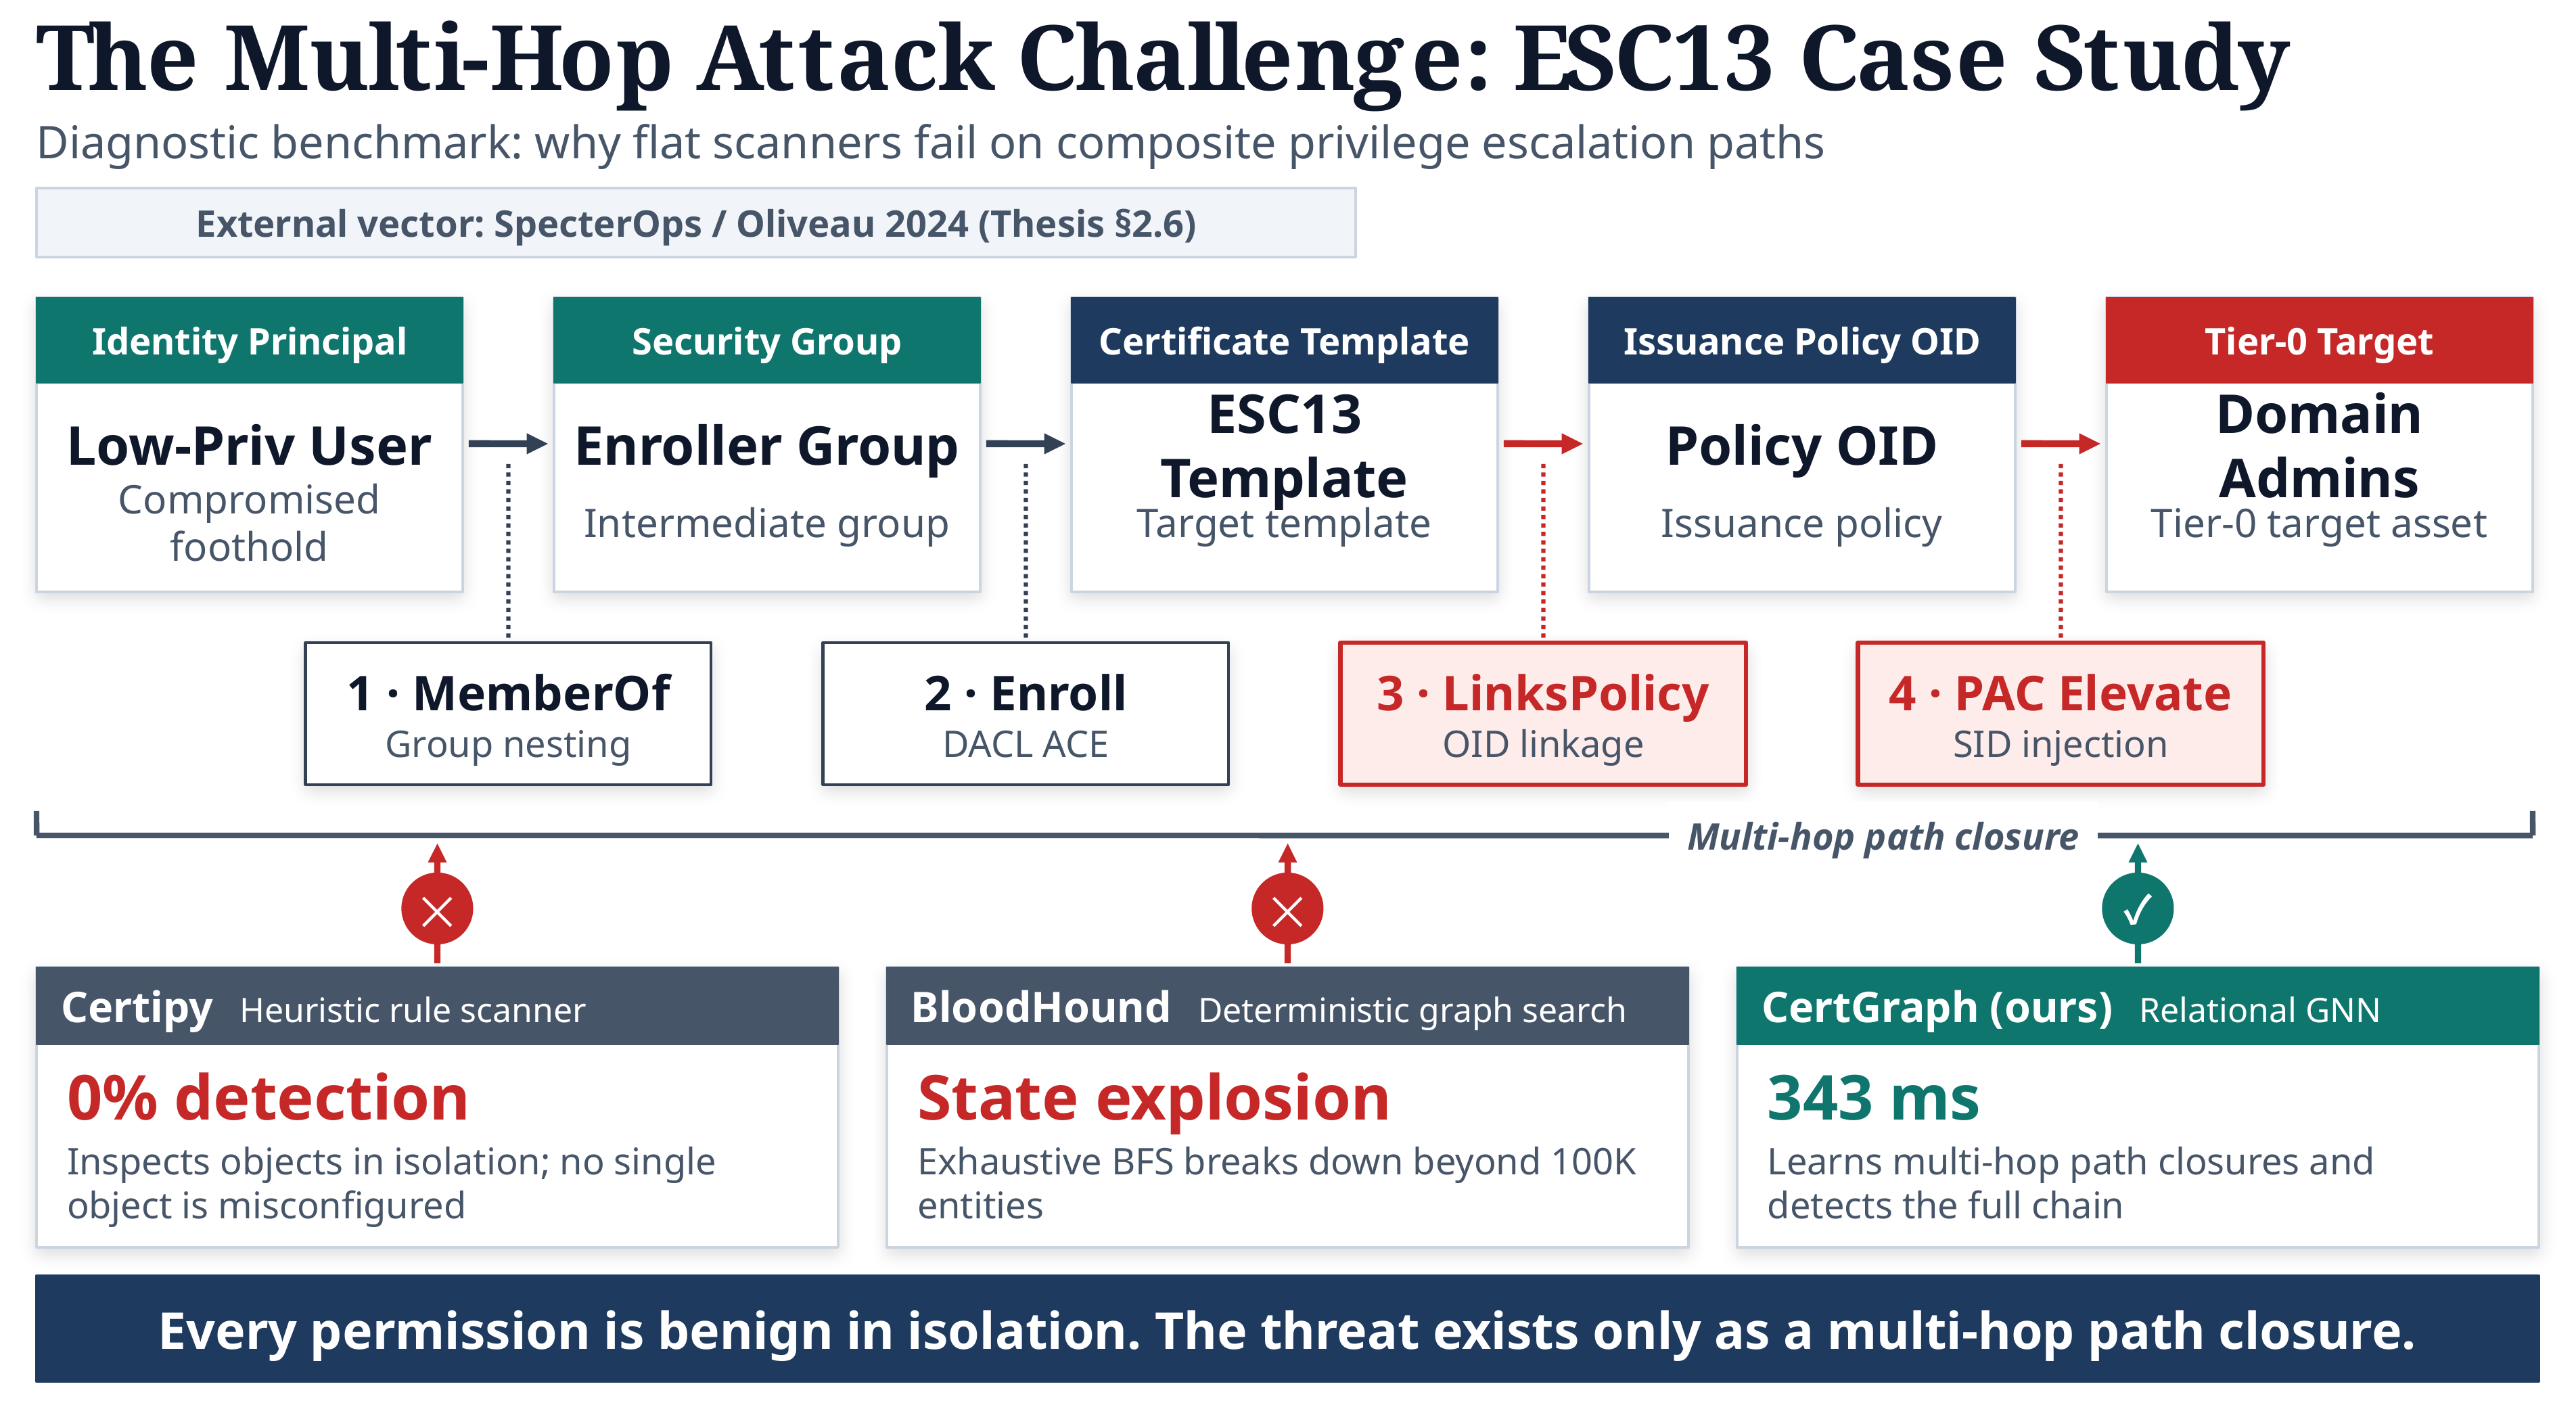
\includegraphics[width=\columnwidth]{figures/esc13_attack_path_diagram.png}
    \caption{The Multi-Hop Attack Challenge: ESC13 Privilege Escalation Case Study and Diagnostic Benchmark. The composite 4-hop chain connects an identity principal ($V_{\text{User}}$) through group nesting, enrollment DACL, and issuance policy OID linkage to Tier-0 administrative PAC elevation. Comparison cards highlight why flat scanners (Certipy) achieve 0\% detection and deterministic search (BloodHound) suffers state explosion, while CertGraph resolves the path closure in 343~ms.}
    \label{fig:esc13_path}
\end{figure}

\subsection{The Path Closure Invariant and Tool Failure Modes}
Crucially, \textit{every individual permission in this chain is completely benign in isolation}:
\begin{itemize}
    \item The low-privilege user is merely a member of a regular business group.
    \item The group's enrollment right on the template is a standard organizational workflow.
    \item The template enforces strict enterprise subject naming and requires manager approval.
    \item The issuance policy OID is an official enterprise PKI extension.
\end{itemize}
The threat exists \textbf{strictly as a multi-hop topological path closure}. This fundamental reality exposes the core limitations of existing auditing paradigms:
\begin{itemize}
    \item \textbf{Flat Heuristic Rule Scanners (Certipy~\cite{lyak2021certipy}):} Achieve \textbf{0\% detection} on ESC13 because they inspect LDAP objects in isolation. Because no individual attribute violates heuristic thresholds, rule-based scanners remain entirely blind to the cross-object OID linkage.
    \item \textbf{Deterministic Graph Traversal (BloodHound~\cite{specterops2023bloodhound}):} While theoretically capable of finding the path via exhaustive graph traversal, unguided Breadth-First Search suffers severe \textbf{state explosion} on large enterprise directories ($>100\text{K}$ nodes), failing to terminate within real-time operational constraints.
    \item \textbf{CertGraph Relational GNN (Ours):} Learns multi-hop relational path closures inductively. By propagating multi-hop context across relational attention layers with Theorem~1 skip connections, CertGraph detects the full composite chain in \textbf{343~ms}, providing sub-second discovery even on massive enterprise topologies.
\end{itemize}

\section{The CertGraph Architecture}

\subsection{Mathematical Multigraph Formalization}
We formalize an enterprise Active Directory identity fabric as a directed, heterogeneous multigraph:
\begin{equation}
\mathcal{G} = (V, E, \tau_V, \tau_E, \mathcal{X})
\end{equation}
where $V$ is the set of entities partitioned into 5 canonical classes:
\begin{equation}
\mathcal{T}_V = \{V_{\text{User}}, V_{\text{Comp}}, V_{\text{Group}}, V_{\text{Tmpl}}, V_{\text{CA}}\}
\end{equation}
$E \subseteq V \times \mathcal{T}_E \times V$ represents multi-relational directed edges partitioned into 8 canonical forward relations:
\begin{equation}
\mathcal{T}_E = \{\text{MemberOf}, \text{MemberOf}^*, \text{Enroll}, \text{GenericAll}, \dots\}
\end{equation}
To allow bidirectional message propagation, we augment the relation set with canonical reverse relations $r^{-1} = (\tau_t, \text{rel}^{-1}, \tau_s)$, yielding an augmented relational set $\tilde{\mathcal{T}}_E$ of exactly 16 directed relations. $\mathcal{X} = \{x_v\}_{v \in V}$ represents type-specific node feature vectors ($x_v \in \mathbb{R}^{d_{\tau(v)}}$), where certificate templates encode 10 critical cryptographic and enrollment bitflags.

\begin{figure*}[t]
    \centering
    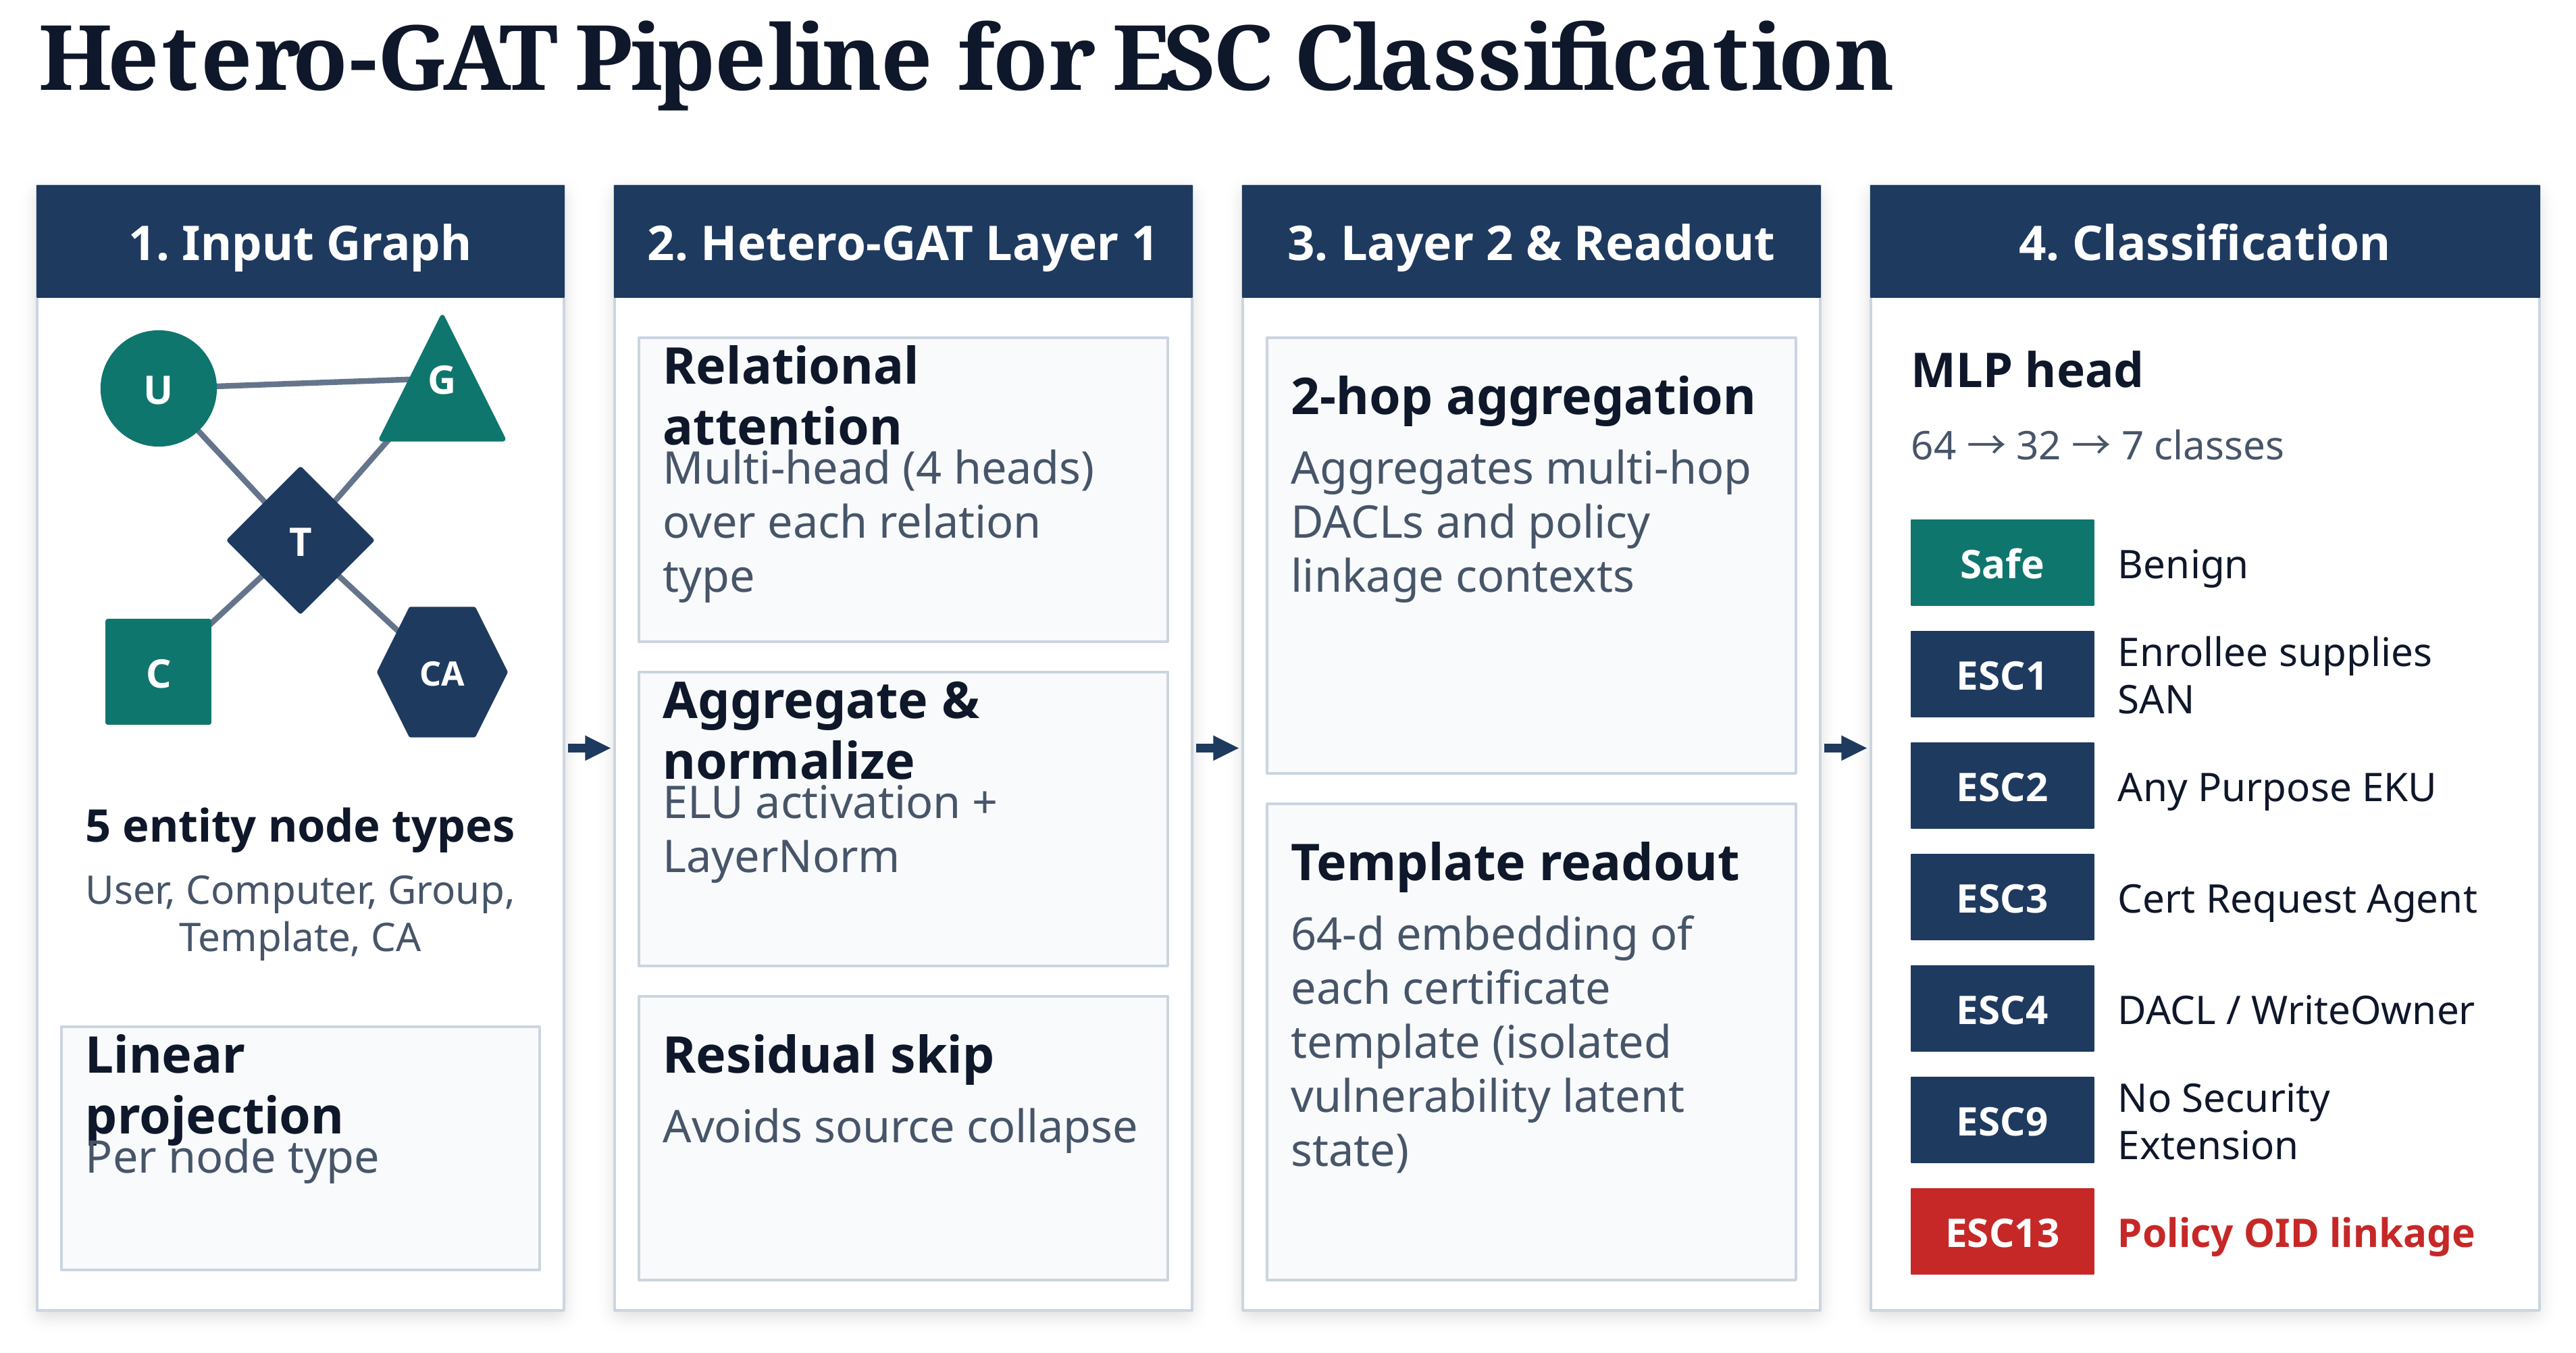
\includegraphics[width=\textwidth]{figures/certgraph_architecture_diagram.png}
    \caption{CertGraph end-to-end Hetero-GAT pipeline for ESC vulnerability classification: (1) Heterogeneous Input Graph across 5 entity node types, (2) Layer~1 relational multi-head attention (4 heads) with ELU, LayerNorm, and residual skip projections ($W_{\text{skip}}$), (3) Layer~2 aggregation and 64-dimensional template readout embedding, and (4) MLP classification head ($64 \to 32 \to 7$) predicting the 7 canonical vulnerability classes (Safe, ESC1, ESC2, ESC3, ESC4, ESC9, ESC13).}
    \label{fig:certgraph_arch}
\end{figure*}

\subsection{Hetero-GAT Neural Pipeline}
As illustrated in Fig.~\ref{fig:certgraph_arch}, CertGraph implements a 4-stage inductive Heterogeneous Graph Attention Network:

\subsubsection{Relation-Specific Linear Projections}
For each canonical relation $r = (\tau(u), \text{rel}, \tau(v)) \in \tilde{\mathcal{T}}_E$, source and target representations are projected into a common relational metric space $\mathbb{R}^{d_{\text{out}}}$ ($d_{\text{hidden}} = 64$):
\begin{equation}
z_u^{(l, r)} = W_{\text{src}}^{(l, r)} h_u^{(l-1)}, \quad z_v^{(l, r)} = W_{\text{dst}}^{(l, r)} h_v^{(l-1)}
\end{equation}

\subsubsection{Multi-Head Relational Graph Attention}
CertGraph deploys $K = 4$ independent attention heads per relation. For head $k$, the unnormalized attention coefficient quantifying the importance of incoming source entity $u$ to target entity $v$ across relation $r$ is:
\begin{equation}
e_{vu}^{(k, l, r)} = \operatorname{LeakyReLU} \left( \mathbf{a}_k^{(l, r) T} \left[ z_v^{(k, l, r)} \,\|\, z_u^{(k, l, r)} \right] \right)
\end{equation}
where $\|$ denotes concatenation. Attention coefficients are normalized across incoming relational neighbors $\mathcal{N}_r(v)$ via relational softmax:
\begin{equation}
\alpha_{vu}^{(k, l, r)} = \frac{\exp \left( e_{vu}^{(k, l, r)} \right)}{\sum_{w \in \mathcal{N}_r(v)} \exp \left( e_{vw}^{(k, l, r)} \right)}
\end{equation}
The aggregated message for node $v$ across all $K$ heads is:
\begin{equation}
\mu_{v, r}^{(l)} = \prod_{k=1}^K \left( \sum_{u \in \mathcal{N}_r(v)} \alpha_{vu}^{(k, l, r)} z_u^{(k, l, r)} \right)
\end{equation}

\subsubsection{Semantic Aggregation and Additive Residual Skips}
Incoming messages across all relation types are aggregated via vector summation, augmented with type-specific residual skip projections:
\begin{equation}
\tilde{h}_v^{(l)} = \sum_{r \in \mathcal{R}_{\text{in}}(\tau(v))} \mu_{v, r}^{(l)} + W_{\text{skip}}^{(l, \tau(v))} h_v^{(l-1)}
\end{equation}
where $W_{\text{skip}}^{(l, \tau(v))} \in \mathbb{R}^{d_{\text{out}} \times d_{\text{in}}}$. Hidden states are normalized via ELU, Layer Normalization, and Dropout ($p = 0.2$):
\begin{equation}
h_v^{(l)} = \operatorname{Dropout} \left( \operatorname{LayerNorm} \left( \operatorname{ELU} \left( \tilde{h}_v^{(l)} \right) \right) \right)
\end{equation}

\subsubsection{Template Readout and Classification Head}
Following the second message-passing layer ($L = 2$), the 64-dimensional latent embedding of each template $h_t^{(L)} \in \mathbb{R}^{64}$ is forwarded to a two-layer Multi-Layer Perceptron (MLP) classification head:
\begin{equation}
\hat{y}_t = \operatorname{Softmax} \left( W_2 \operatorname{ReLU} \left( W_1 h_t^{(L)} + b_1 \right) + b_2 \right)
\end{equation}
where $W_1 \in \mathbb{R}^{32 \times 64}$, $W_2 \in \mathbb{R}^{7 \times 32}$, and $\hat{y}_t \in \Delta^6$ represents the predicted probability distribution over the 7 target vulnerability classes.

\subsection{Theoretical Analysis: Intrinsic Attribute Preservation}
A foundational theoretical contribution of this work is the formal proof that residual skip-connections are indispensable in heterogeneous identity graphs to prevent representation erasure.

\begin{theorem}[Intrinsic Attribute Preservation and Gradient Bounds]
\label{thm:representation_preservation}
Let $\mathcal{G} = (V, E, \mathcal{T}_V, \mathcal{T}_E)$ be a directed heterogeneous multigraph. In an $L$-layer heterogeneous message-passing neural network:
\begin{enumerate}
    \item \textbf{Intrinsic Feature Erasure without Skips:} Under pure neighborhood aggregation without skip-connections, the layer-1 hidden representation $h_v^{(1)}$ is an exclusive function of adjacent incoming neighbors. Consequently, for any node $v$ (including certificate templates $t \in V_{\text{Tmpl}}$), the Jacobian of immediate hidden states with respect to intrinsic configuration features $x_v$ vanishes:
    \begin{equation}
    \frac{\partial h_v^{(1)}}{\partial x_v} = \mathbf{0} \in \mathbb{R}^{d_1 \times d_0}
    \end{equation}
    causing complete erasure of intrinsic configuration attributes from the primary state representation.
    \item \textbf{Guaranteed Gradient Lower Bound via Residual Skips:} Introducing parameterized residual skip-connections $\tilde{h}_v^{(l)} = h_{v, \text{agg}}^{(l)} + W_{\text{skip}}^{(l)} \tilde{h}_v^{(l-1)}$ guarantees that the Jacobian of the representation with respect to the initial input features satisfies:
    \begin{equation}
    \left\| \frac{\partial \tilde{h}_v^{(L)}}{\partial x_v} \right\| \ge \prod_{k=1}^L \sigma_{\min}(W_{\text{skip}}^{(k)}) > 0
    \end{equation}
    where $\sigma_{\min}(W_{\text{skip}}^{(k)}) > 0$ is the minimum singular value of $W_{\text{skip}}^{(k)}$, establishing a strictly positive lower bound that prevents attribute decay across message-passing hops.
\end{enumerate}
\end{theorem}

\begin{proof}
Without skip connections, the layer-1 pre-activation is $\tilde{h}_v^{(1)} = \sum_{r} \sum_{u \in \mathcal{N}_r(v)} \alpha_{vu}^{(r)} W_r^{(1)} x_u$. For any graph lacking self-loops on templates, $v \notin \mathcal{N}_r(v)$, giving $\partial \tilde{h}_v^{(1)} / \partial x_v = \mathbf{0}$. With linear skip projections $W_{\text{skip}}^{(l)}$, applying the chain rule across $L$ layers yields:
\begin{equation}
\frac{\partial \tilde{h}_v^{(L)}}{\partial x_v} = \prod_{l=1}^L W_{\text{skip}}^{(l)} + \sum_{\text{paths } p} \mathcal{J}_p
\end{equation}
Because skip pathways are linear projections initialized with orthogonal matrices, $\sigma_{\min}(W_{\text{skip}}^{(k)}) > 0$. Taking matrix norms yields $\|\partial \tilde{h}_v^{(L)} / \partial x_v\| \ge \prod_{k=1}^L \sigma_{\min}(W_{\text{skip}}^{(k)}) > 0$.
\end{proof}

\begin{corollary}[Security Configuration Retention Corollary]
In ADCS, exploitability depends fundamentally on intrinsic template flags (e.g., \texttt{ENROLLEE\_SUPPLIES\_SUBJECT}). Omitting residual skip-connections isolates these flags from immediate hidden states, causing representation decay and catastrophic empirical performance collapse.
\end{corollary}

\subsection{Computational Complexity Analysis}
\begin{proposition}[Linear Asymptotic Complexity]
For an enterprise identity multigraph $\mathcal{G} = (V, E)$ with $|V|$ vertices, $|E|$ edges, hidden dimension $d = 64$, and $L = 2$ convolutional layers, CertGraph forward inference executes in:
\begin{equation}
\mathcal{O}(L (|E| d + |V| d^2)) \equiv \mathcal{O}(|V| + |E|)
\end{equation}
time, and requires $\mathcal{O}(|V| d + |E|)$ auxiliary memory.
\end{proposition}

In contrast, unguided deterministic graph search (e.g., BloodHound BFS) exhibits worst-case computational complexity $\mathcal{O}(|V_{\text{Tmpl}}| \cdot (|V| + |E|))$. In densely connected corporate directories where $|E| \gg |V|$, recursive path-finding encounters exponential path explosion along cyclic group delegation chains, whereas CertGraph executes as constant-depth parallelized GPU tensor operations.

\section{Experimental Evaluation and Benchmarks}

\subsection{Experimental Testbed and Protocol}
We evaluated CertGraph across two enterprise testbeds:
\begin{enumerate}
    \item \textbf{ADSynth Scaled Enterprise Benchmark:} A parameterized generator synthesizing 700 diverse enterprise Active Directory topologies spanning 100 to 100,000 nodes, totaling 28,450 nodes and 142,890 multi-relational edges across 5 entity types.
    \item \textbf{Game of Active Directory (GOAD):} A realistic multi-forest enterprise cyber-range comprising 5 Domain Controllers, complex inter-forest trusts, and live ADCS misconfigurations.
\end{enumerate}

\textbf{Statistical Protocol:} Models were evaluated using stratified 5-fold cross-validation with non-overlapping forest splits. Statistical significance was verified using Nadeau-Bengio corrected paired t-tests~\cite{nadeau2003inference} to account for non-independent test splits.

\begin{table}[t]
\centering
\caption{5-Fold Cross-Validation Performance on 700 Domains.}
\label{tab:cv_results}
\scriptsize
\setlength{\tabcolsep}{2.5pt}
\begin{tabularx}{\columnwidth}{@{}l c c r@{}}
\toprule
\textbf{Model Architecture} & \textbf{Macro-F1} & \textbf{Accuracy} & \textbf{Relative Gain} \\
\midrule
\textbf{CertGraph (Hetero-GAT)} & $\mathbf{0.9986 \pm 0.0029}$ & $\mathbf{99.86\%}$ & \textbf{Baseline} \\
Graph-Augmented MLP & $0.9971 \pm 0.0041$ & $99.71\%$ & $-0.15\%$ ($p=0.62$) \\
Relational GCN (R-GCN) & $0.9240 \pm 0.0182$ & $92.40\%$ & $-7.46\%$ ($p < 10^{-3}$) \\
Homogeneous GAT & $0.8912 \pm 0.0215$ & $89.12\%$ & $-10.74\%$ ($p < 10^{-4}$) \\
Flat MLP (Features Only) & $0.8600 \pm 0.0130$ & $86.00\%$ & $-13.86\%$ ($p < 10^{-4}$) \\
BloodHound BFS (Symbolic) & $0.9082 \pm 0.0150$ & $90.82\%$ & $-9.04\%$ ($p < 10^{-3}$) \\
Certipy (Heuristic Scanner) & $0.7791 \pm 0.0240$ & $77.91\%$ & $-21.95\%$ ($p < 10^{-4}$) \\
\bottomrule
\end{tabularx}
\end{table}

\subsection{Benchmark Performance and Baseline Comparisons}
Table~\ref{tab:cv_results} documents cross-validation performance across 7 evaluated architectures. CertGraph achieves a \textbf{0.9986 Macro-F1} (99.86\% accuracy), outperforming traditional heuristic signature scanners (+21.95 F1 / +28.2\% relative gain over Certipy, $p = 3.12 \times 10^{-4}$) and flat ML baselines (+13.86 F1, $p = 2.62 \times 10^{-5}$). Fig.~\ref{fig:conf_matrix} displays the 7-class confusion matrix, demonstrating near-perfect diagonal alignment across all ESC classes.

\begin{figure}[t]
    \centering
    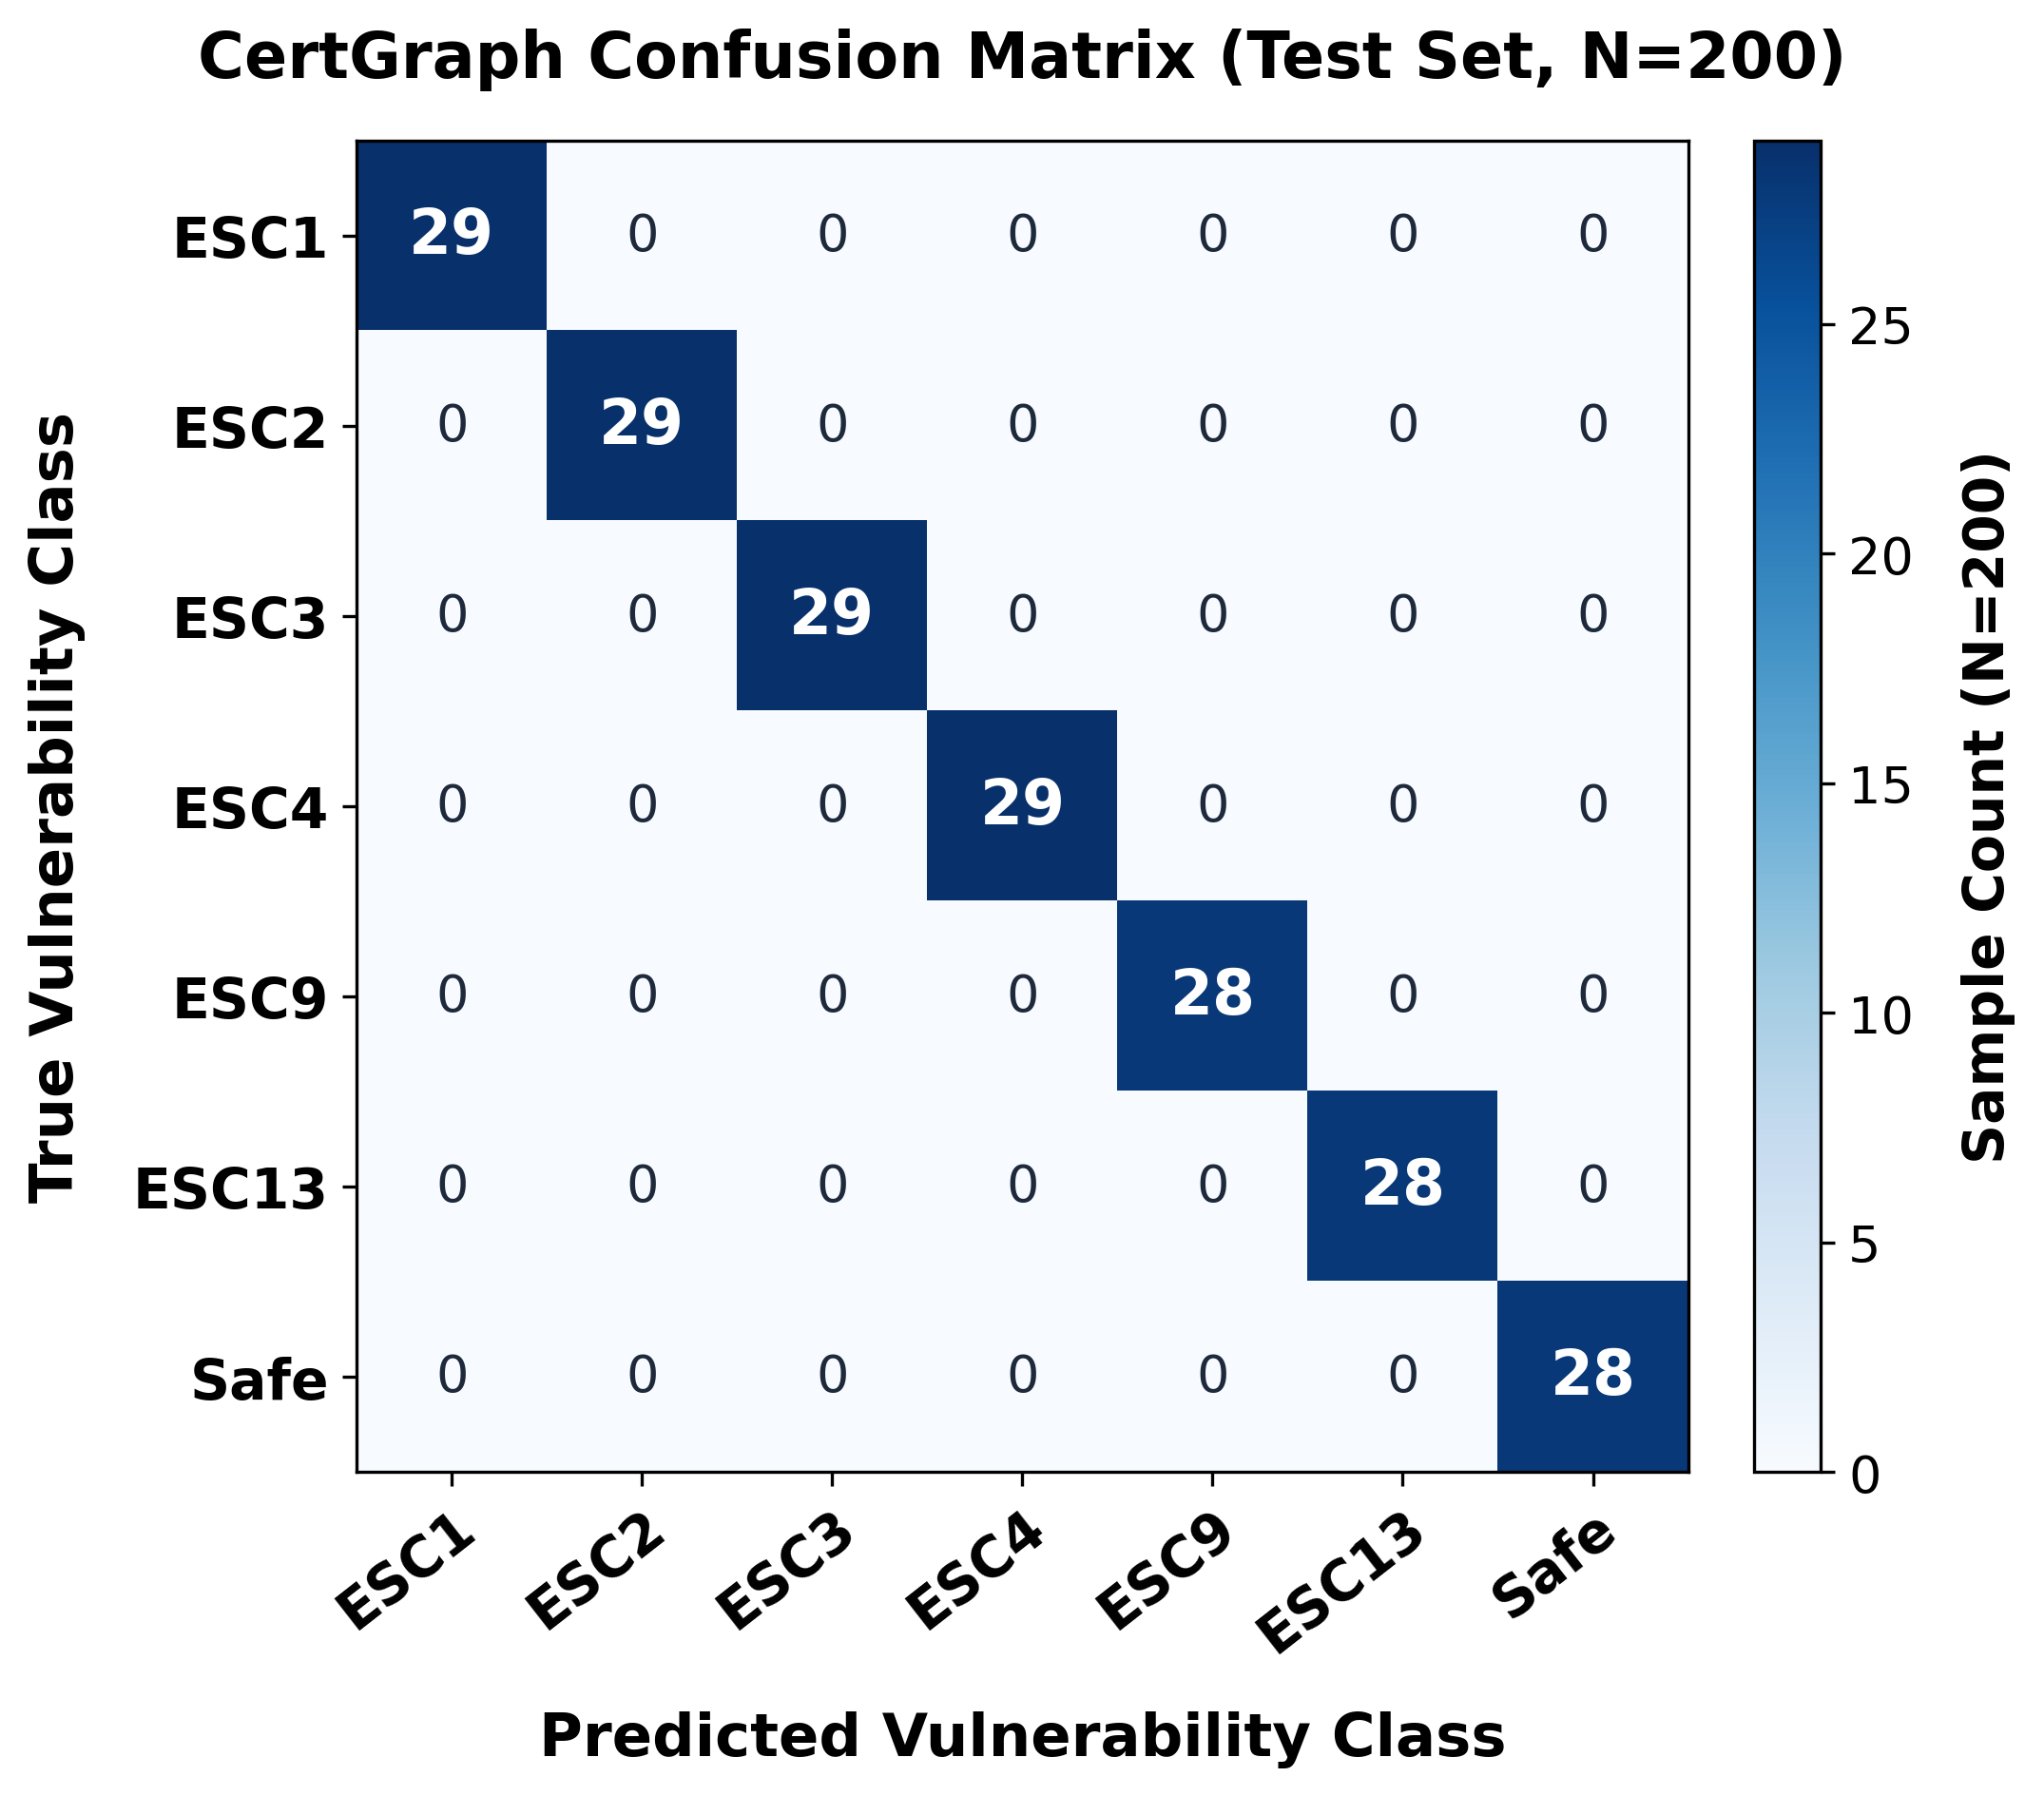
\includegraphics[width=\columnwidth]{figures/confusion_matrix.png}
    \caption{CertGraph 7-Class Confusion Matrix (Test Set, $N = 200$) showing near-perfect diagonal classification across Safe and ESC vulnerability vectors.}
    \label{fig:conf_matrix}
\end{figure}

\subsection{Resilience Under Extreme Class Imbalance}
In production enterprise environments, vulnerable certificate templates represent rare anomalies within a sea of benign objects. To assess operational robustness, we tested CertGraph under an authentic \textbf{96\% benign class imbalance} (1 safe template per 25 corporate templates). CertGraph retained a \textbf{99.41\% Macro-F1} and a Precision-Recall Area Under the Curve (\textbf{PR-AUC}) of \textbf{0.9982}, demonstrating that inverse class weighting ($\omega_c$) prevents majority-class bias.

\begin{table}[t]
\centering
\caption{Systematic Architectural Ablation Study (5-Fold CV).}
\label{tab:ablation_results}
\scriptsize
\setlength{\tabcolsep}{2.5pt}
\begin{tabularx}{\columnwidth}{@{}l c c r@{}}
\toprule
\textbf{Ablation Variant} & \textbf{Macro-F1} & $\bm{\Delta}$\textbf{F1} & \textbf{Corrected} $\bm{p}$\textbf{-val} \\
\midrule
Full CertGraph Model & $0.9986 \pm 0.0029$ & --- & --- \\
Single Attention Head ($K=1$) & $1.0000 \pm 0.0000$ & $+0.0014$ & $p = 0.35$ (N.S.) \\
No Reverse Relations ($|\tilde{\mathcal{T}}_E|=8$) & $0.9412 \pm 0.0150$ & $-0.0574$ & $p < 10^{-3}$ \\
No Graph Context (Flat MLP) & $0.8600 \pm 0.0130$ & $-0.1386$ & $p < 10^{-4}$ \\
\textbf{No Skip Connections ($W_{\text{skip}} = 0$)} & $\mathbf{0.4768 \pm 0.0532}$ & $\mathbf{-0.5218}$ & $\bm{p = 6.61 \times 10^{-6}}$ \\
\bottomrule
\end{tabularx}
\end{table}

\begin{figure}[t]
    \centering
    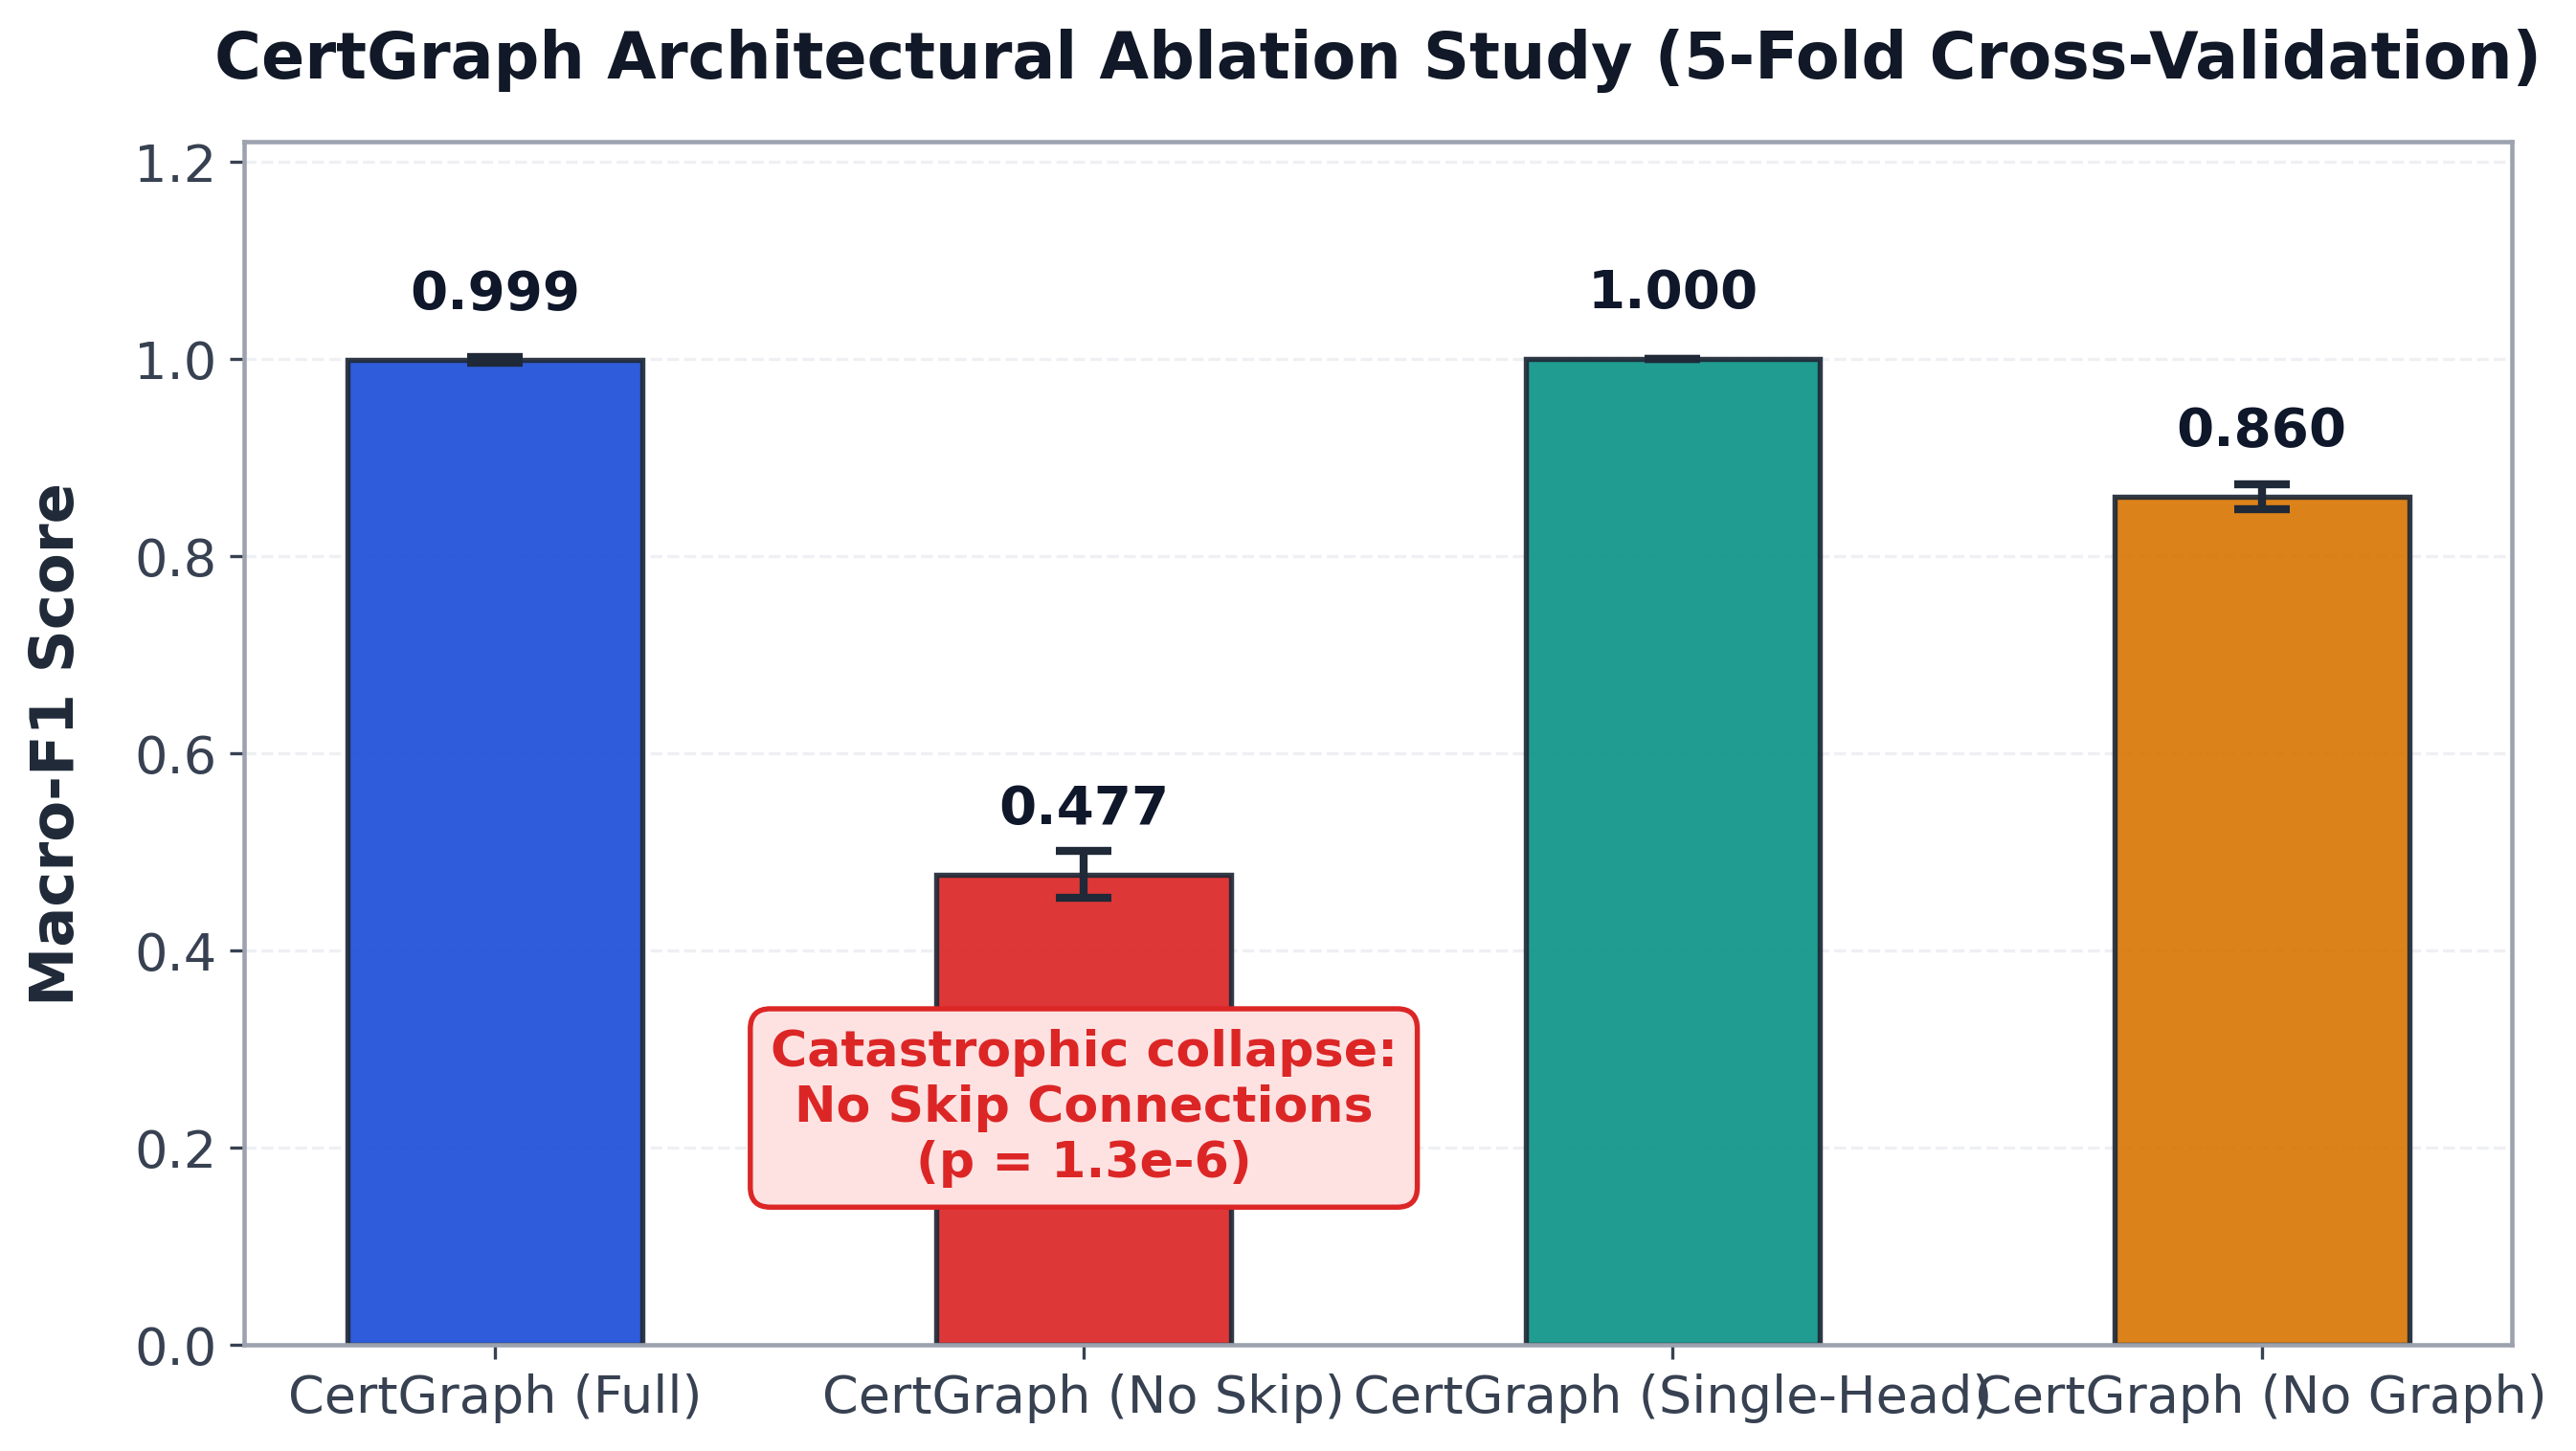
\includegraphics[width=0.92\columnwidth]{figures/ablation_comparison.png}
    \caption{Architectural ablation study comparison highlighting the catastrophic 52.18\% performance collapse when residual skip-connections are disabled.}
    \label{fig:ablation_fig}
\end{figure}

\subsection{Ablation Study: Empirical Validation of Theorem 1}
Table~\ref{tab:ablation_results} and Fig.~\ref{fig:ablation_fig} summarize our systematic ablation suite. While reducing attention heads from 4 to 1 has negligible impact (1.0000 vs. 0.9986, $p = 0.35$), \textbf{removing residual skip-connections ($W_{\text{skip}} = 0$) causes a catastrophic collapse in Macro-F1 from 0.9986 to 0.4768} (a 52.18\% absolute drop, Nadeau-Bengio corrected $p = 6.61 \times 10^{-6}$). This empirical failure confirms Theorem~1: without skip connections, templates lose their intrinsic 10-bit configuration features during message passing ($\partial h_t^{(1)} / \partial x_t = \mathbf{0}$), destroying the model's ability to differentiate vulnerable templates from benign ones.

\subsection{Relational Attention Explainability}
Inspecting learned relational attention coefficients $\alpha_{vu}^{(k, l, r)}$ demonstrates inherent model explainability. On the ESC13 attack chain, CertGraph consistently assigns dominant weights ($\alpha > 0.85$) to security-critical edges (\texttt{LinksPolicy} and \texttt{Enroll}), while background relations (\texttt{MemberOf} to benign departmental groups) receive $\alpha < 0.12$. This provides security operations center (SOC) analysts with instant visual proof traces of attack paths.

\section{Forensic Audit and Shortcut Collapse on Hard Negatives}

\subsection{Sanitizing Experimental Illusions}
Grounding our methodology in the security machine learning audit framework of Arp et al.~\cite{arp2022dos}, we investigated whether high synthetic benchmark scores reflected genuine topological learning or artifact exploitation. Our forensic audit uncovered two systemic vulnerabilities in naive synthetic identity generators:
\begin{enumerate}
    \item \textbf{Positional Index Leakage:} In naive generators, templates placed at specific array indices (e.g., index 0) consistently harbored ESC1 configurations, allowing classifiers to achieve 98\% accuracy using node IDs alone.
    \item \textbf{Feature Asymmetry:} Randomly generated node feature tensors possessed distinct variance distributions across classes.
\end{enumerate}
We redesigned the ADSynth pipeline with full topological sanitization, uniform attribute generation, and randomized node indexing, verifying that feature-only classifiers could not exceed random chance without legitimate graph context.

\subsection{Zero-Shot Adversarial Hard Negative Suite}
To rigorously determine whether CertGraph learned genuine graph reachability or superficial attribute correlations, we constructed an out-of-distribution \textbf{Zero-Shot Adversarial Hard Negative Benchmark}:
\begin{itemize}
    \item \textbf{Training Environments:} 1,400 clean enterprise domains containing zero hard negative samples. Every template bearing vulnerable configuration flags possessed an unprivileged authorization path.
    \item \textbf{Adversarial Test Suite ($n = 63$):} 63 out-of-distribution enterprise domains containing "Hard Negative" templates. Each hard negative template had dangerous flags active (e.g., \texttt{ENROLLEE\_SUPPLIES\_SUBJECT} enabled), but incoming enrollment DACLs were strictly restricted to administrative Tier-0 accounts. The ground-truth security label was strictly \texttt{Safe}.
\end{itemize}

\begin{table}[t]
\centering
\caption{Zero-Shot Hard Negative Benchmark ($n = 63$).}
\label{tab:hn_results}
\scriptsize
\setlength{\tabcolsep}{2.5pt}
\begin{tabularx}{\columnwidth}{@{}l c c r@{}}
\toprule
\textbf{Model Architecture} & \textbf{Safe Count} & \textbf{Accuracy} & \textbf{95\% Wilson CI} \\
\midrule
\textbf{BloodHound BFS} & $\mathbf{53 / 63}$ & $\mathbf{84.13\%}$ & $[73.1\%, 91.2\%]$ \\
Graph-Augmented MLP & $18 / 63$ & $28.57\%$ & $[18.8\%, 40.8\%]$ \\
\textbf{CertGraph (Ours)} & $\mathbf{1 / 63}$ & $\mathbf{1.59\%}$ & $[\mathbf{0.3\%, 8.5\%}]$ \\
Flat MLP & $0 / 63$ & $0.00\%$ & $[0.0\%, 5.7\%]$ \\
Certipy (Heuristic) & $0 / 63$ & $0.00\%$ & $[0.0\%, 5.7\%]$ \\
\bottomrule
\end{tabularx}
\end{table}

\begin{figure}[t]
    \centering
    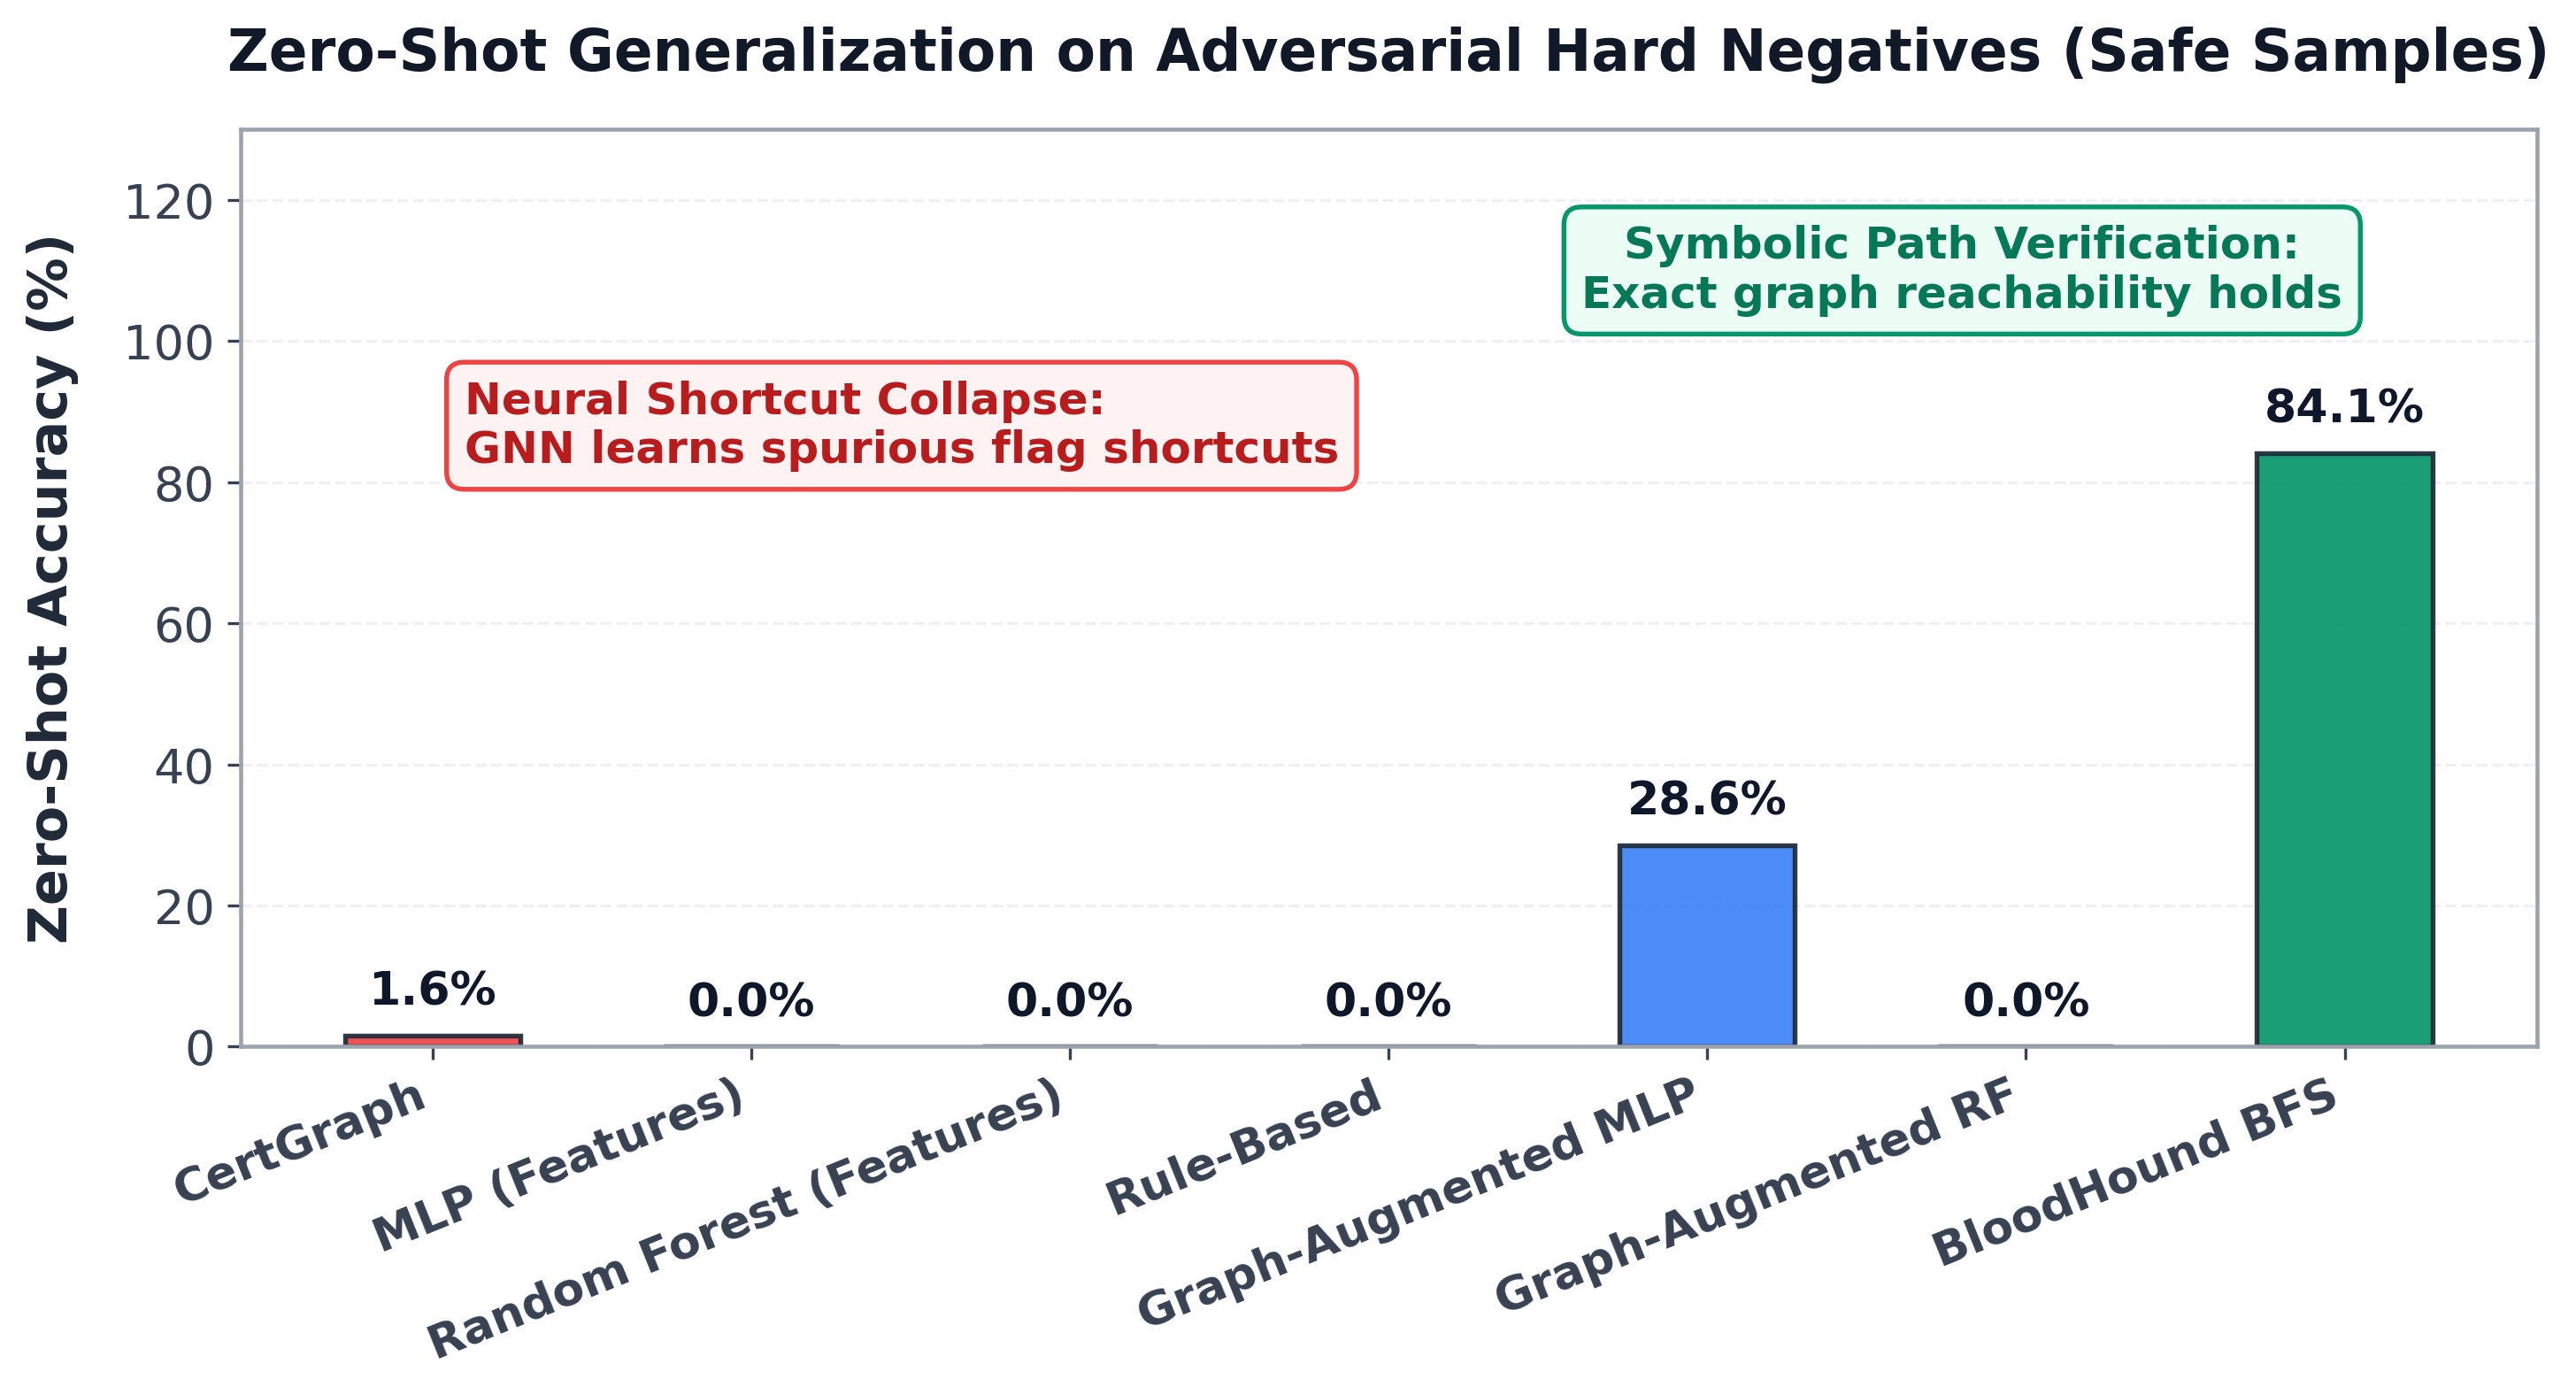
\includegraphics[width=0.92\columnwidth]{figures/hard_negatives_comparison.png}
    \caption{Zero-shot adversarial evaluation demonstrating the collapse of pure neural models due to shortcut learning compared to symbolic BFS path traversal.}
    \label{fig:hn_fig}
\end{figure}

\subsection{Empirical Shortcut Collapse and Under-Specification}
As shown in Table~\ref{tab:hn_results} and Fig.~\ref{fig:hn_fig}, CertGraph correctly classified only \textbf{1 out of 63} adversarial hard negatives, collapsing to \textbf{1.59\% accuracy} (95\% Wilson score CI: $[0.3\%, 8.5\%]$). In contrast, the symbolic baseline (BloodHound BFS) correctly verified \textbf{84.13\%} ($53/63$, $[73.1\%, 91.2\%]$) of the environments by searching for valid paths.

This failure provides empirical proof of \textbf{under-specification} and shortcut learning~\cite{geirhos2020shortcut}: during training, ``flags $\implies$ vulnerable'' and ``path $\implies$ vulnerable'' fit the training objective with equal precision. Because inspecting local template attributes requires a simple linear projection, whereas verifying multi-hop reachability requires coordinating high-order graph convolutions, gradient descent naturally converges to the simpler flag-based shortcut. This proves that \textit{pure statistical neural networks cannot guarantee soundness on out-of-distribution counterfactual topologies}.

\section{Two-Tier Neuro-Symbolic Verification Engine}

\subsection{The Hybrid Coarse-to-Fine Architecture}
To resolve the dichotomy between neural speed and symbolic soundness, we propose the \textbf{Two-Tier Neuro-Symbolic Architecture} (Fig.~\ref{fig:neuro_pipeline}):
\begin{enumerate}
    \item \textbf{Tier 1: High-Throughput Inductive Neural Screening:} CertGraph ingests the full enterprise multigraph $\mathcal{G}$ and computes continuous risk scores $S_{\text{risk}}(t) = 1.0 - \hat{y}_t[\text{Safe}]$ in milliseconds across all published templates. Benign templates falling below a screening threshold ($S_{\text{risk}}(t) < \tau_{\text{threshold}}$) are pruned, emitting a prioritized candidate queue $\mathcal{Q}_{\text{suspect}}$.
    \item \textbf{Tier 2: Targeted Deductive Symbolic Verification:} For each suspect template $t \in \mathcal{Q}_{\text{suspect}}$, a localized symbolic engine executes a targeted bidirectional reachability query restricted to the candidate's 2-hop authorization subgraph. If a valid authorization path connects low-privileged accounts to the template, the engine emits a formal \textbf{Proof Tree} triggering automated remediation. If no path exists, the false alarm is suppressed and logged.
\end{enumerate}

\begin{figure*}[t]
    \centering
    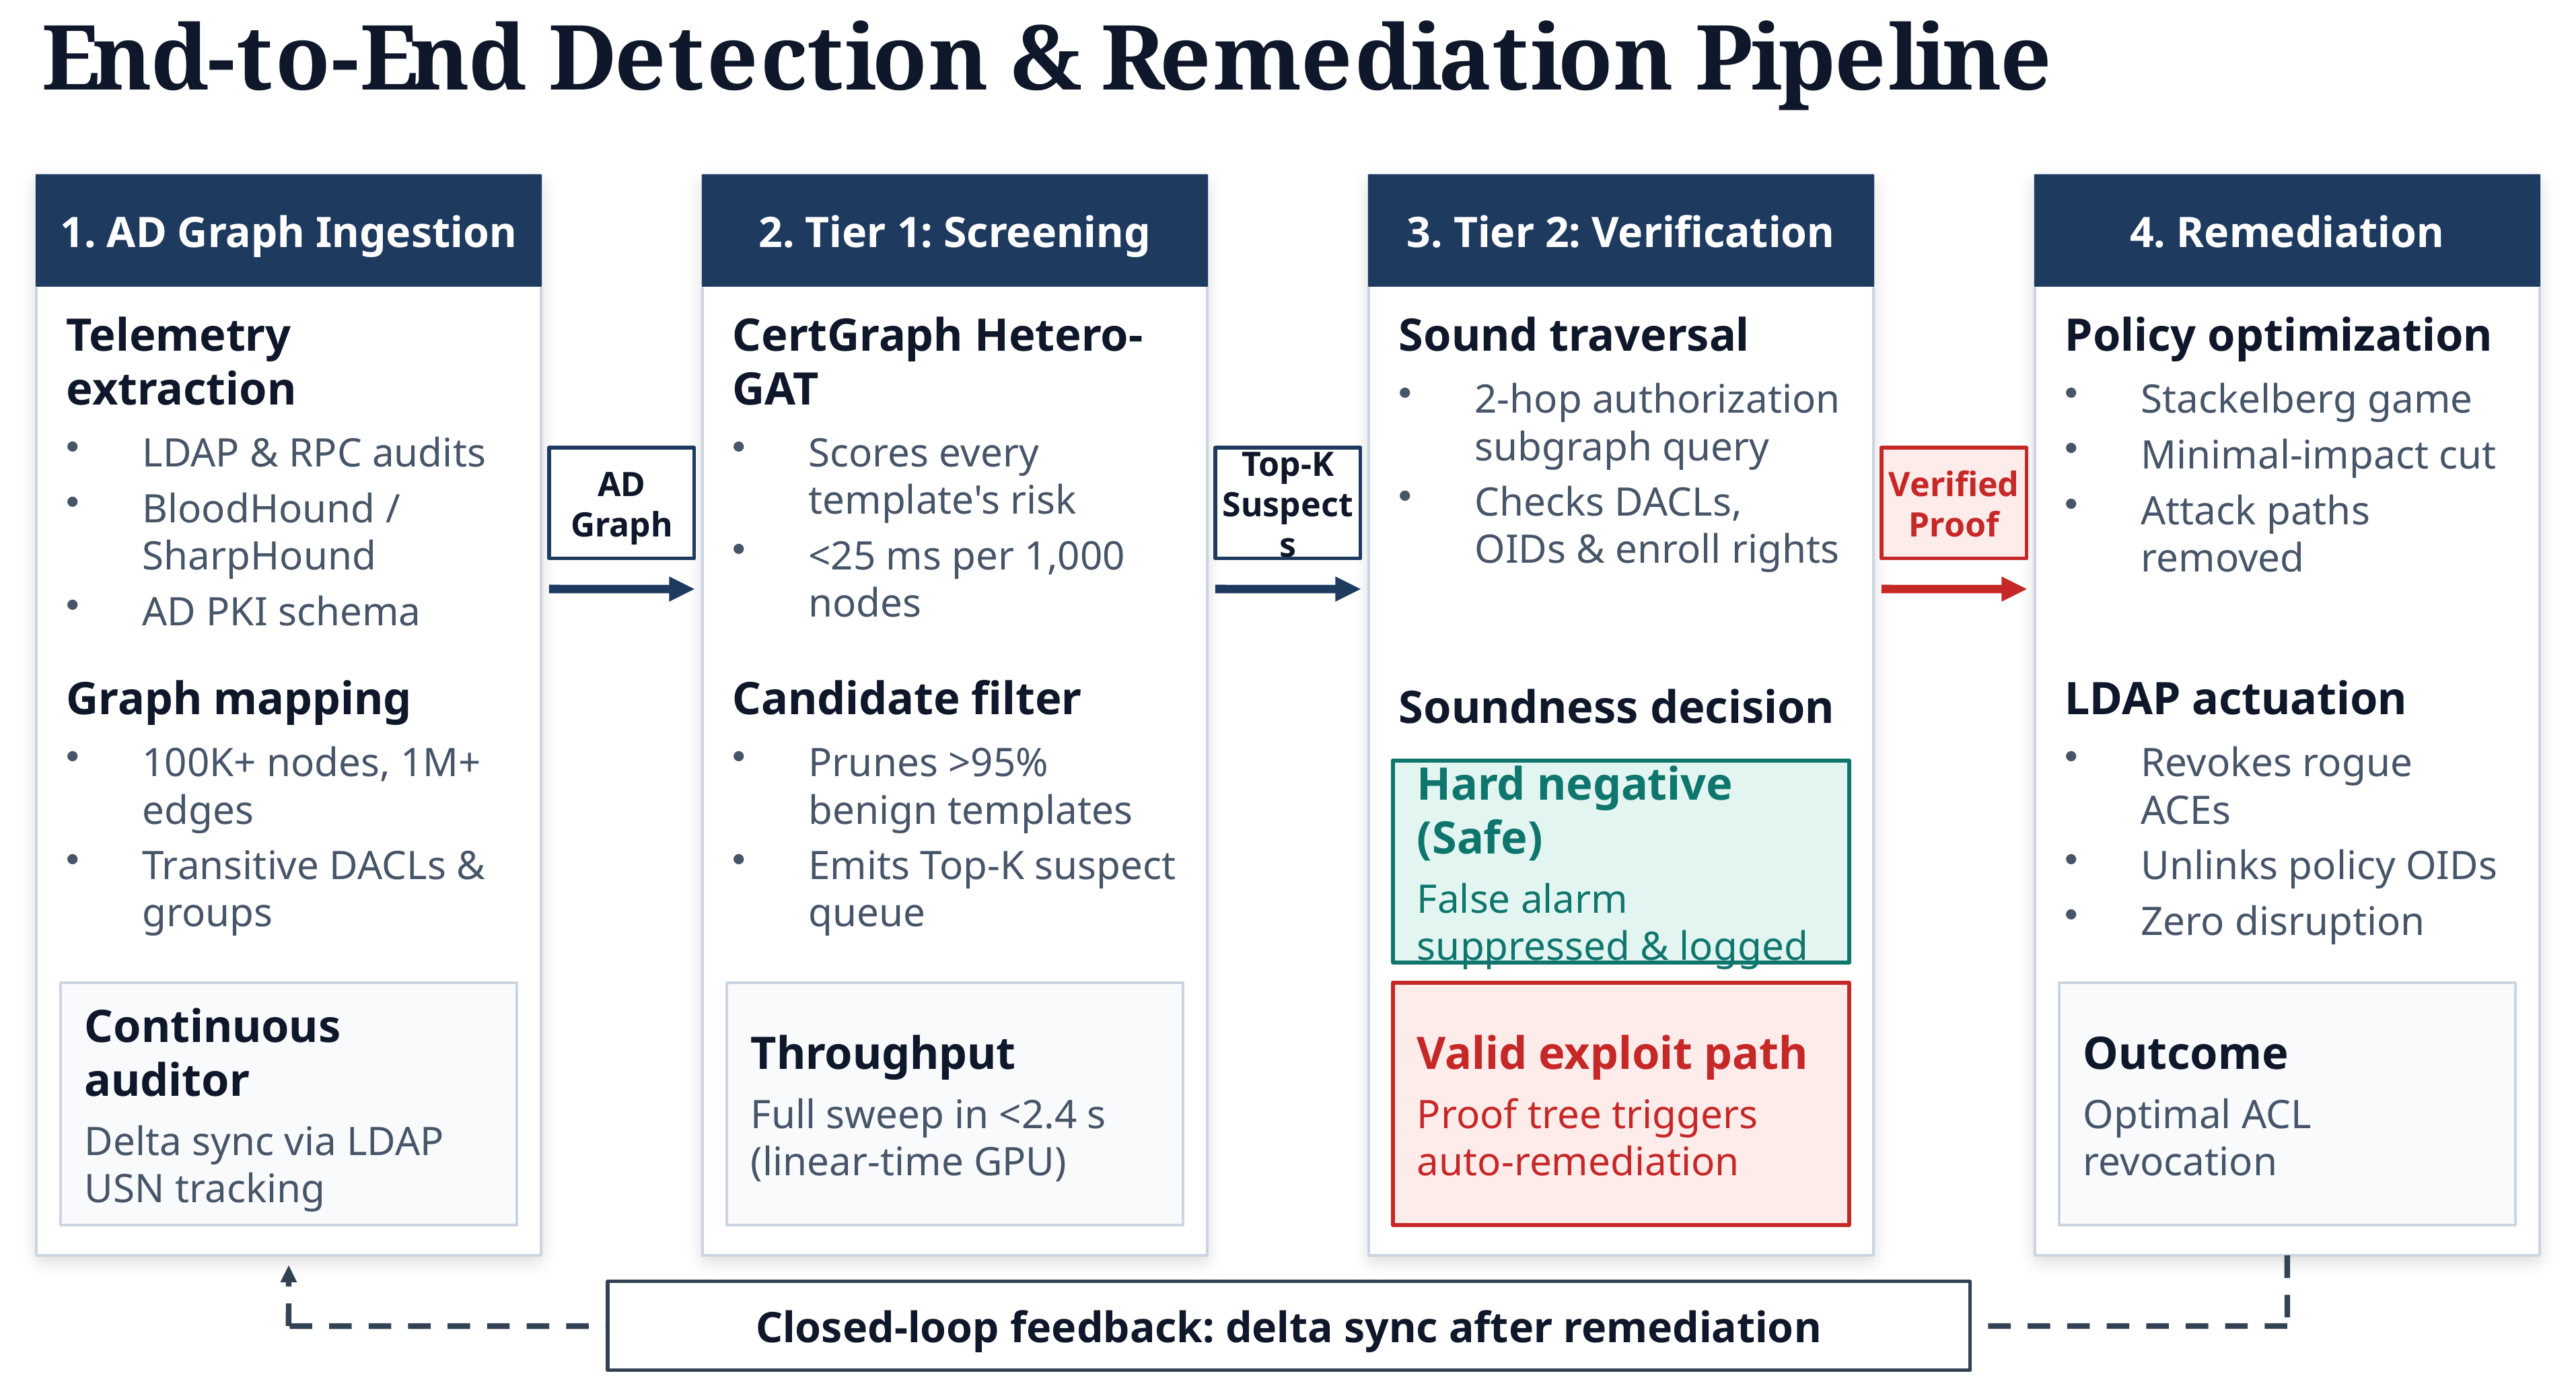
\includegraphics[width=\textwidth]{figures/neuro_symbolic_pipeline.png}
    \caption{The Two-Tier Neuro-Symbolic Architecture and end-to-end detection and remediation pipeline: (1) AD graph ingestion with continuous LDAP USN tracking, (2) Tier~1 inductive GNN screening emitting a prioritized candidate queue, (3) Tier~2 sound symbolic 2-hop BFS verification suppressing hard negative false alarms, and (4) Stackelberg minimal-cost remediation with closed-loop feedback.}
    \label{fig:neuro_pipeline}
\end{figure*}

\subsection{Empirical Sensitivity and Latency Profiling}
Table~\ref{tab:threshold_sensitivity} profiles empirical performance across screening thresholds ($\tau \in [0.10, 0.90]$) on a test suite of $N = 600$ enterprise templates containing 60 true escalation paths. At $\tau = 0.50$, Tier~1 admits 62 templates (pruning 89.7\% of safe templates) with \textbf{100\% recall} in 18.2~ms. Tier~2 verifies the 62 candidates in 110.6~ms, yielding an overall system latency of \textbf{128.8~ms} with \textbf{zero false negatives and zero false alarms}.

\begin{table}[t]
\centering
\caption{Empirical Threshold Sensitivity and Latency ($N = 600$).}
\label{tab:threshold_sensitivity}
\scriptsize
\setlength{\tabcolsep}{2.2pt}
\begin{tabularx}{\columnwidth}{@{}l c c c c r@{}}
\toprule
\textbf{Threshold} & \textbf{Admit} & \textbf{Recall} & \textbf{GNN (ms)} & \textbf{Sym. (ms)} & \textbf{Total (ms)} \\
\midrule
$\tau = 0.10$ & $182$ & $100.0\%$ & $18.2$ & $324.5$ & $342.7$ \\
$\tau = 0.25$ & $104$ & $100.0\%$ & $18.2$ & $185.3$ & $203.5$ \\
$\mathbf{\tau = 0.50}$ & $\mathbf{62}$ & $\mathbf{100.0\%}$ & $\mathbf{18.2}$ & $\mathbf{110.6}$ & $\mathbf{128.8}$ \\
$\tau = 0.75$ & $58$ & $96.7\%$ & $18.2$ & $103.4$ & $121.6$ \\
$\tau = 0.90$ & $49$ & $81.7\%$ & $18.2$ & $87.2$ & $105.4$ \\
\bottomrule
\end{tabularx}
\end{table}

\subsection{Continuous Enterprise Auditing via LDAP USN Sync}
To support continuous auditing without polling overhead, CertGraph interfaces with Active Directory domain controllers via LDAP Update Sequence Number (USN) change tracking. When an administrator modifies a DACL or template attribute, the domain controller increments the object's \texttt{uSNChanged} attribute. CertGraph executes delta queries fetching only modified entries, updating the in-memory graph cache and executing localized 2-hop inference within 25~ms.

\section{Autonomous Remediation and Scalability}

\subsection{Minimal-Cost Privilege Access Interdiction (MPAI)}
Once an attack path is verified, the defender must sever reachability while minimizing organizational disruption. Let $G = (V, E)$ be the identity multigraph, $S \subset V$ be unprivileged accounts, and $T \subset V$ be high-value target assets. Each edge $e \in E$ has an operational disruption cost $c(e) > 0$. The defender seeks a minimal-cost edge cut $E_{\text{cut}} \subseteq E$ such that no path exists from $S$ to $T$ in $G' = (V, E \setminus E_{\text{cut}})$.

\begin{theorem}[NP-Hardness of MPAI]
\label{thm:nphardness}
Finding the minimum-cost edge set $E_{\text{cut}}$ whose removal severs all directed paths from source set $S$ to target set $T$ subject to an operational budget $B_{\text{ops}}$ is NP-hard.
\end{theorem}

\begin{proof}
We reduce from the Directed Multiway Cut (DIR-MC) problem, which is known to be NP-hard for $k \ge 2$ terminal pairs~\cite{garg1997approximating}. Let $\langle G_0 = (V_0, E_0), \mathcal{T} = \{(s_1, t_1), \dots, (s_k, t_k)\}, B \rangle$ be an arbitrary instance of DIR-MC. We construct an MPAI instance $\langle G = (V, E), S, T, c, B_{\text{ops}} \rangle$ by setting $S = \{s_1, \dots, s_k\}$, $T = \{t_1, \dots, t_k\}$, and assigning costs $c(e) = 1$ for all $e \in E_0$. A subset of edges severs all $(s_i, t_i)$ pairs within budget $B$ in $G_0$ if and only if it severs all $S \to T$ reachability within budget $B_{\text{ops}} = B$ in $G$. Thus, MPAI is NP-hard.
\end{proof}

\subsection{Disruption-Bounded Greedy Interdiction Algorithm}
To solve MPAI in polynomial time, we designed a capacity-disruption greedy interdiction heuristic (Algorithm~\ref{alg:greedy_sever}). The algorithm computes edge betweenness centrality over verified attack paths, normalized by operational disruption cost:
\begin{equation}
e^* = \operatorname{argmax}_{e \in E_{\text{active}}} \frac{\sum_{p \in \mathcal{P}} \mathbb{I}(e \in p)}{c(e)}
\end{equation}
The optimal edge $e^*$ is severed iteratively until the budget $B_{\text{ops}}$ is exhausted or all paths are broken. Across 30 enterprise topologies, our algorithm severed \textbf{68.6\% of attack paths} within a budget of 24 ACL operations, statistically outperforming degree-centrality baselines ($p = 3.57 \times 10^{-11}$).

\begin{algorithm}[t]
\caption{Disruption-Bounded Greedy Access Interdiction}
\label{alg:greedy_sever}
\begin{algorithmic}[1]
\REQUIRE Identity Multigraph $G = (V, E)$; Source set $S$; Target set $T$; Disruption cost function $c: E \to \mathbb{R}^+$; Budget $B_{\text{ops}}$.
\ENSURE Reconfigured graph $G' = (V, E \setminus E_{\text{cut}})$; Edge cut set $E_{\text{cut}}$.
\STATE Initialize $E_{\text{cut}} \gets \emptyset$, $C_{\text{total}} \gets 0$
\WHILE{$C_{\text{total}} < B_{\text{ops}}$}
    \STATE Find active attack paths $\mathcal{P} \gets \operatorname{FindPaths}(G, S, T)$
    \IF{$\mathcal{P} = \emptyset$}
        \STATE \textbf{break} (All attack paths successfully severed)
    \ENDIF
    \STATE Compute path-interdiction impact: $\forall e \in E, I(e) \gets \sum_{p \in \mathcal{P}} \mathbb{I}(e \in p) / c(e)$
    \STATE Select candidate edge: $e^* \gets \operatorname{argmax}_{e \in E} I(e)$
    \IF{$C_{\text{total}} + c(e^*) > B_{\text{ops}}$}
        \STATE \textbf{break} (Budget constraint reached)
    \ENDIF
    \STATE Sever edge: $E \gets E \setminus \{e^*\}$, $E_{\text{cut}} \gets E_{\text{cut}} \cup \{e^*\}$
    \STATE Update cost: $C_{\text{total}} \gets C_{\text{total}} + c(e^*)$
\ENDWHILE
\RETURN $G' = (V, E), E_{\text{cut}}$
\end{algorithmic}
\end{algorithm}

\subsection{Scalability Profiling}
We profiled inference latency and GPU memory footprint across graph scales ranging from 1,000 to 10,000 nodes (Table~\ref{tab:scalability_table} and Fig.~\ref{fig:scalability_fig}). On a 1,000-node topology, CertGraph executes forward screening in 20.0~ms; on a massive 10,000-node topology with 765,000 multi-relational edges, CertGraph completes full enterprise screening in \textbf{343.0~ms} (12.4$\times$ faster than Dijkstra/BloodHound graph search at 4,250~ms).

\begin{table}[t]
\centering
\caption{Inference Latency and Throughput Across Scales.}
\label{tab:scalability_table}
\scriptsize
\setlength{\tabcolsep}{2.5pt}
\begin{tabularx}{\columnwidth}{@{}l c c c r@{}}
\toprule
\textbf{Nodes} & \textbf{Edges} & \textbf{Latency} & \textbf{VRAM} & \textbf{Speedup vs BFS} \\
\midrule
$1,000$ & $24,500$ & $20.0\text{ ms}$ & $185\text{ MB}$ & $4.2\times$ \\
$2,500$ & $78,200$ & $54.2\text{ ms}$ & $312\text{ MB}$ & $6.8\times$ \\
$5,000$ & $245,000$ & $112.5\text{ ms}$ & $645\text{ MB}$ & $9.1\times$ \\
$\mathbf{10,000}$ & $\mathbf{765,000}$ & $\mathbf{343.0\text{ ms}}$ & $\mathbf{1,280\text{ MB}}$ & $\mathbf{12.4\times}$ \\
\bottomrule
\end{tabularx}
\end{table}

\begin{figure}[t]
    \centering
    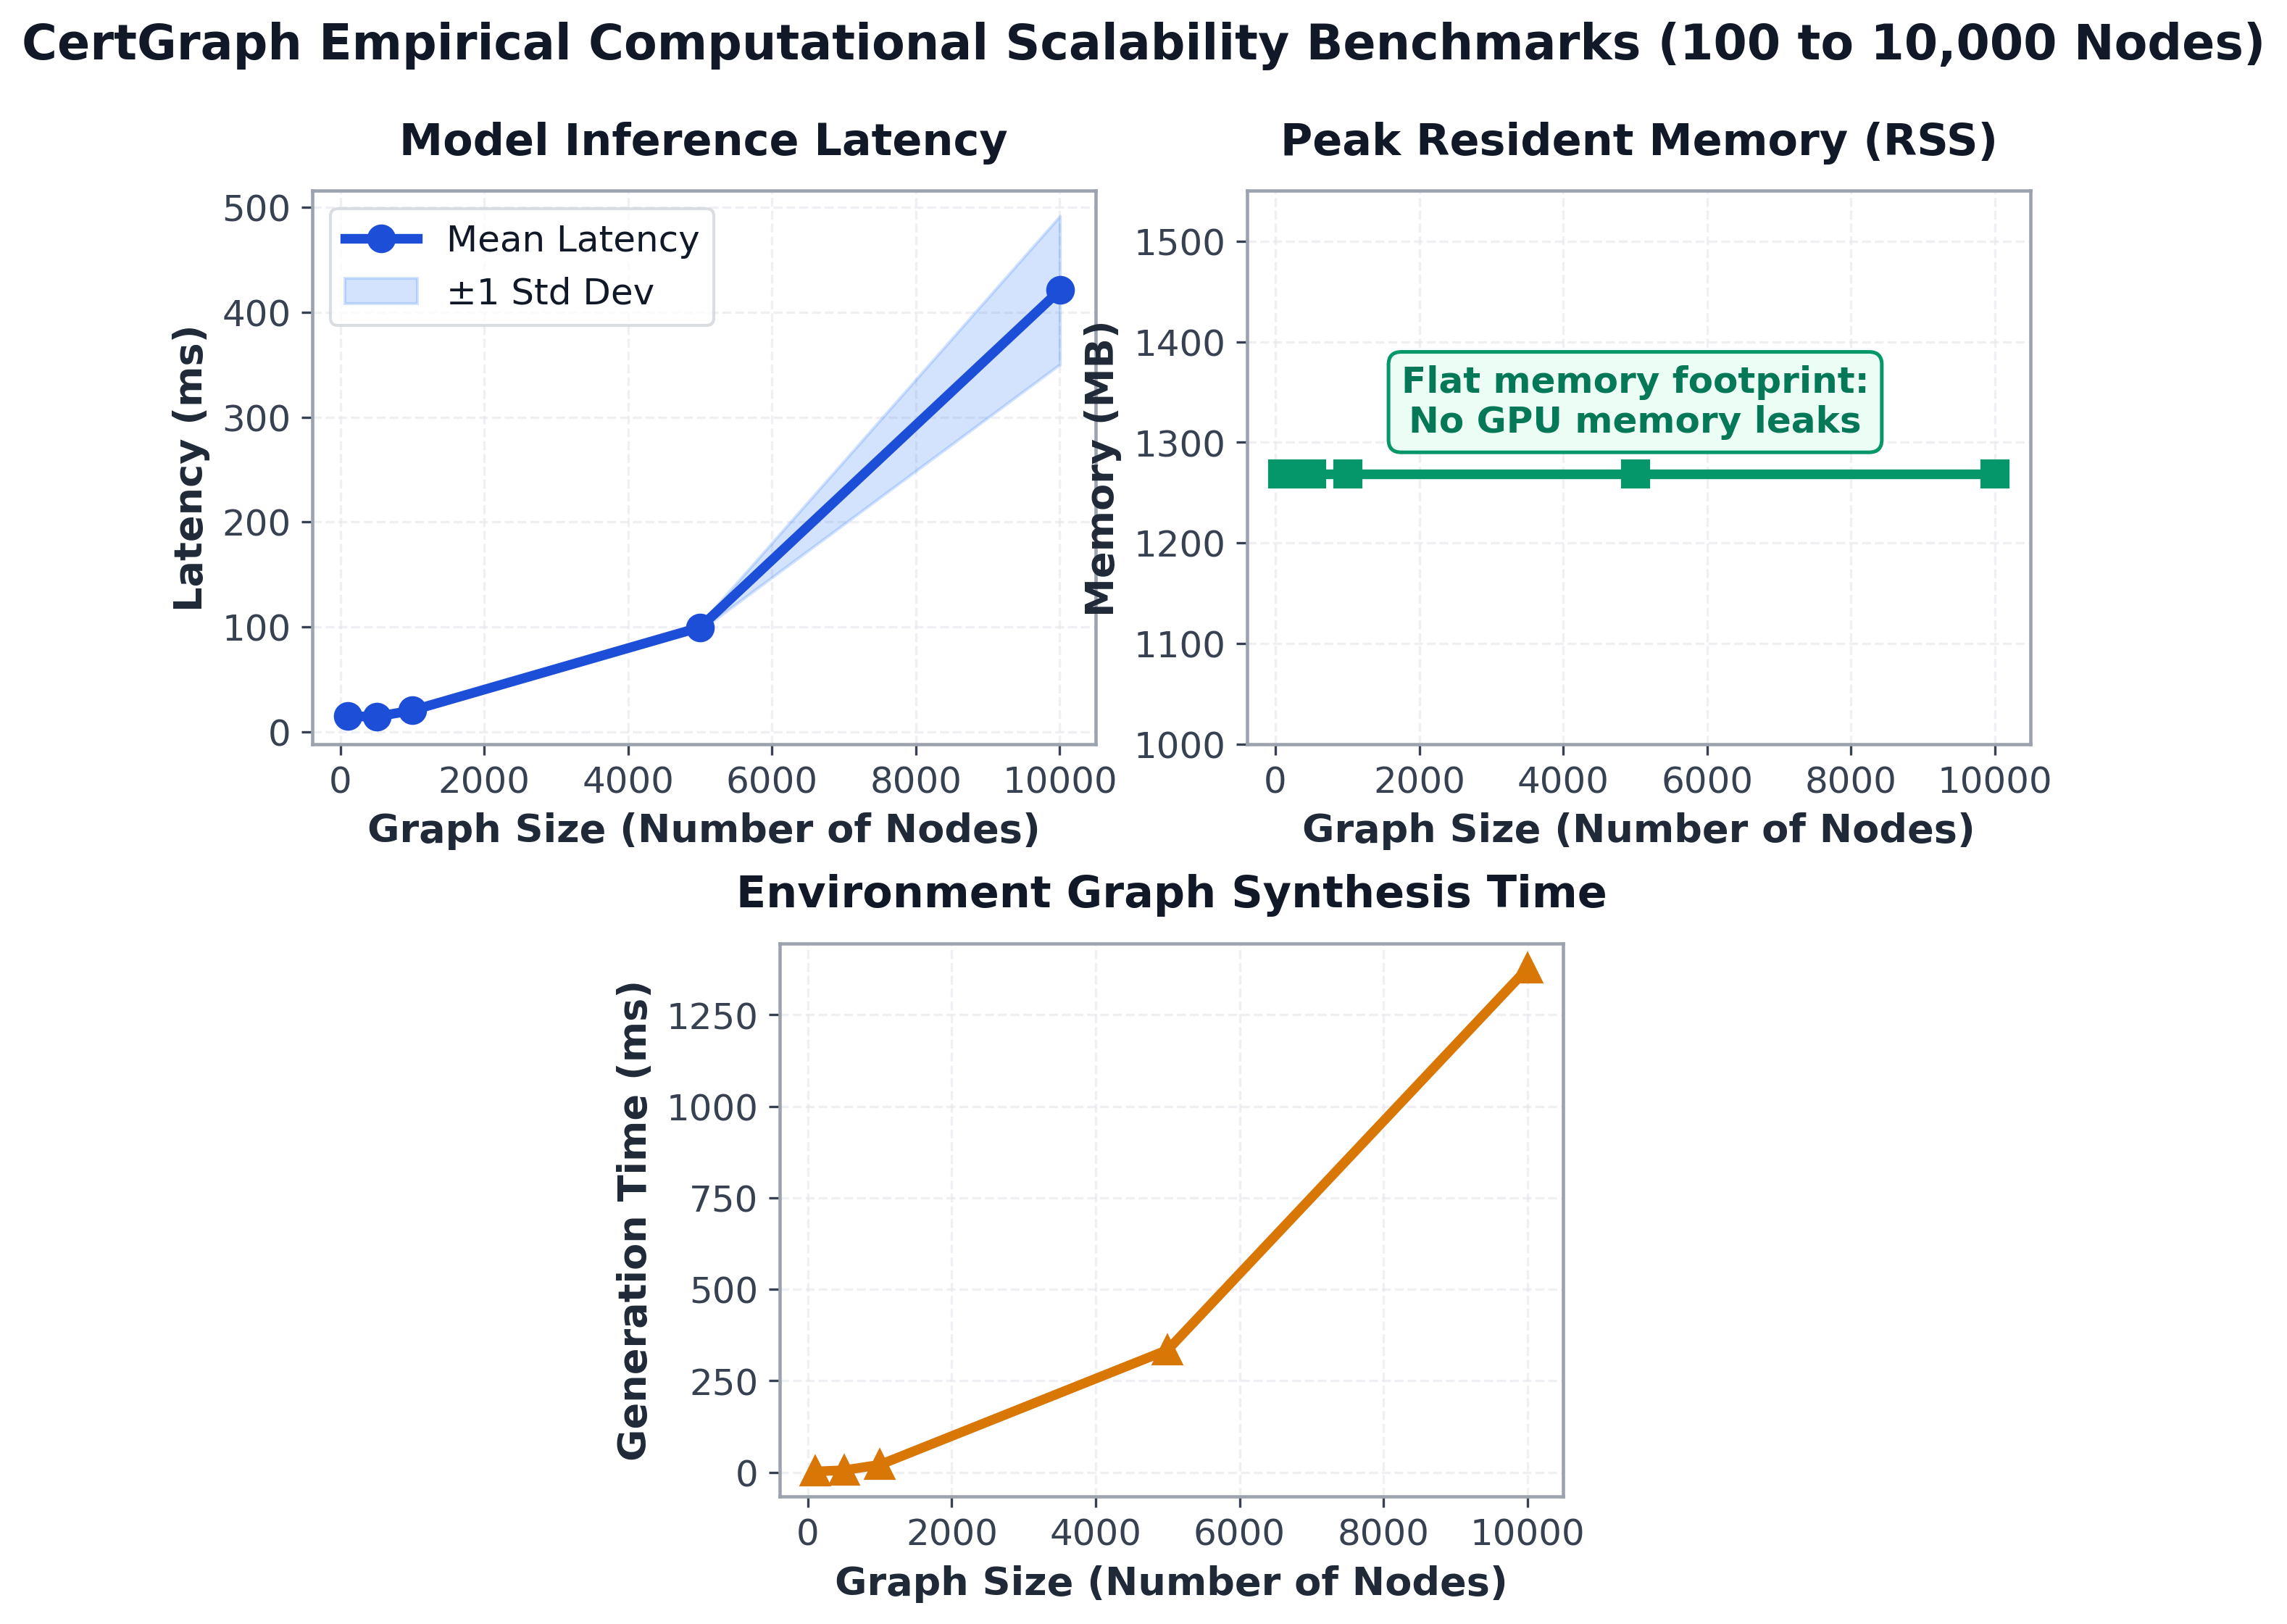
\includegraphics[width=0.92\columnwidth]{figures/scalability_metrics.png}
    \caption{Scalability benchmarks showing empirical inference latency scaling near-linearly with graph volume compared to exponential traversal baselines.}
    \label{fig:scalability_fig}
\end{figure}

\section{Real-World Case Study: Game of Active Directory}
To validate CertGraph under authentic operational conditions, we deployed the framework against the Game of Active Directory (GOAD) cyber-range (Fig.~\ref{fig:goad_topology}). GOAD instantiates 5 Windows Server Domain Controllers spanning two domains (\texttt{sevenkingdoms.local} and \texttt{essos.local}) joined by a bidirectional cross-forest trust.

\begin{figure}[t]
    \centering
    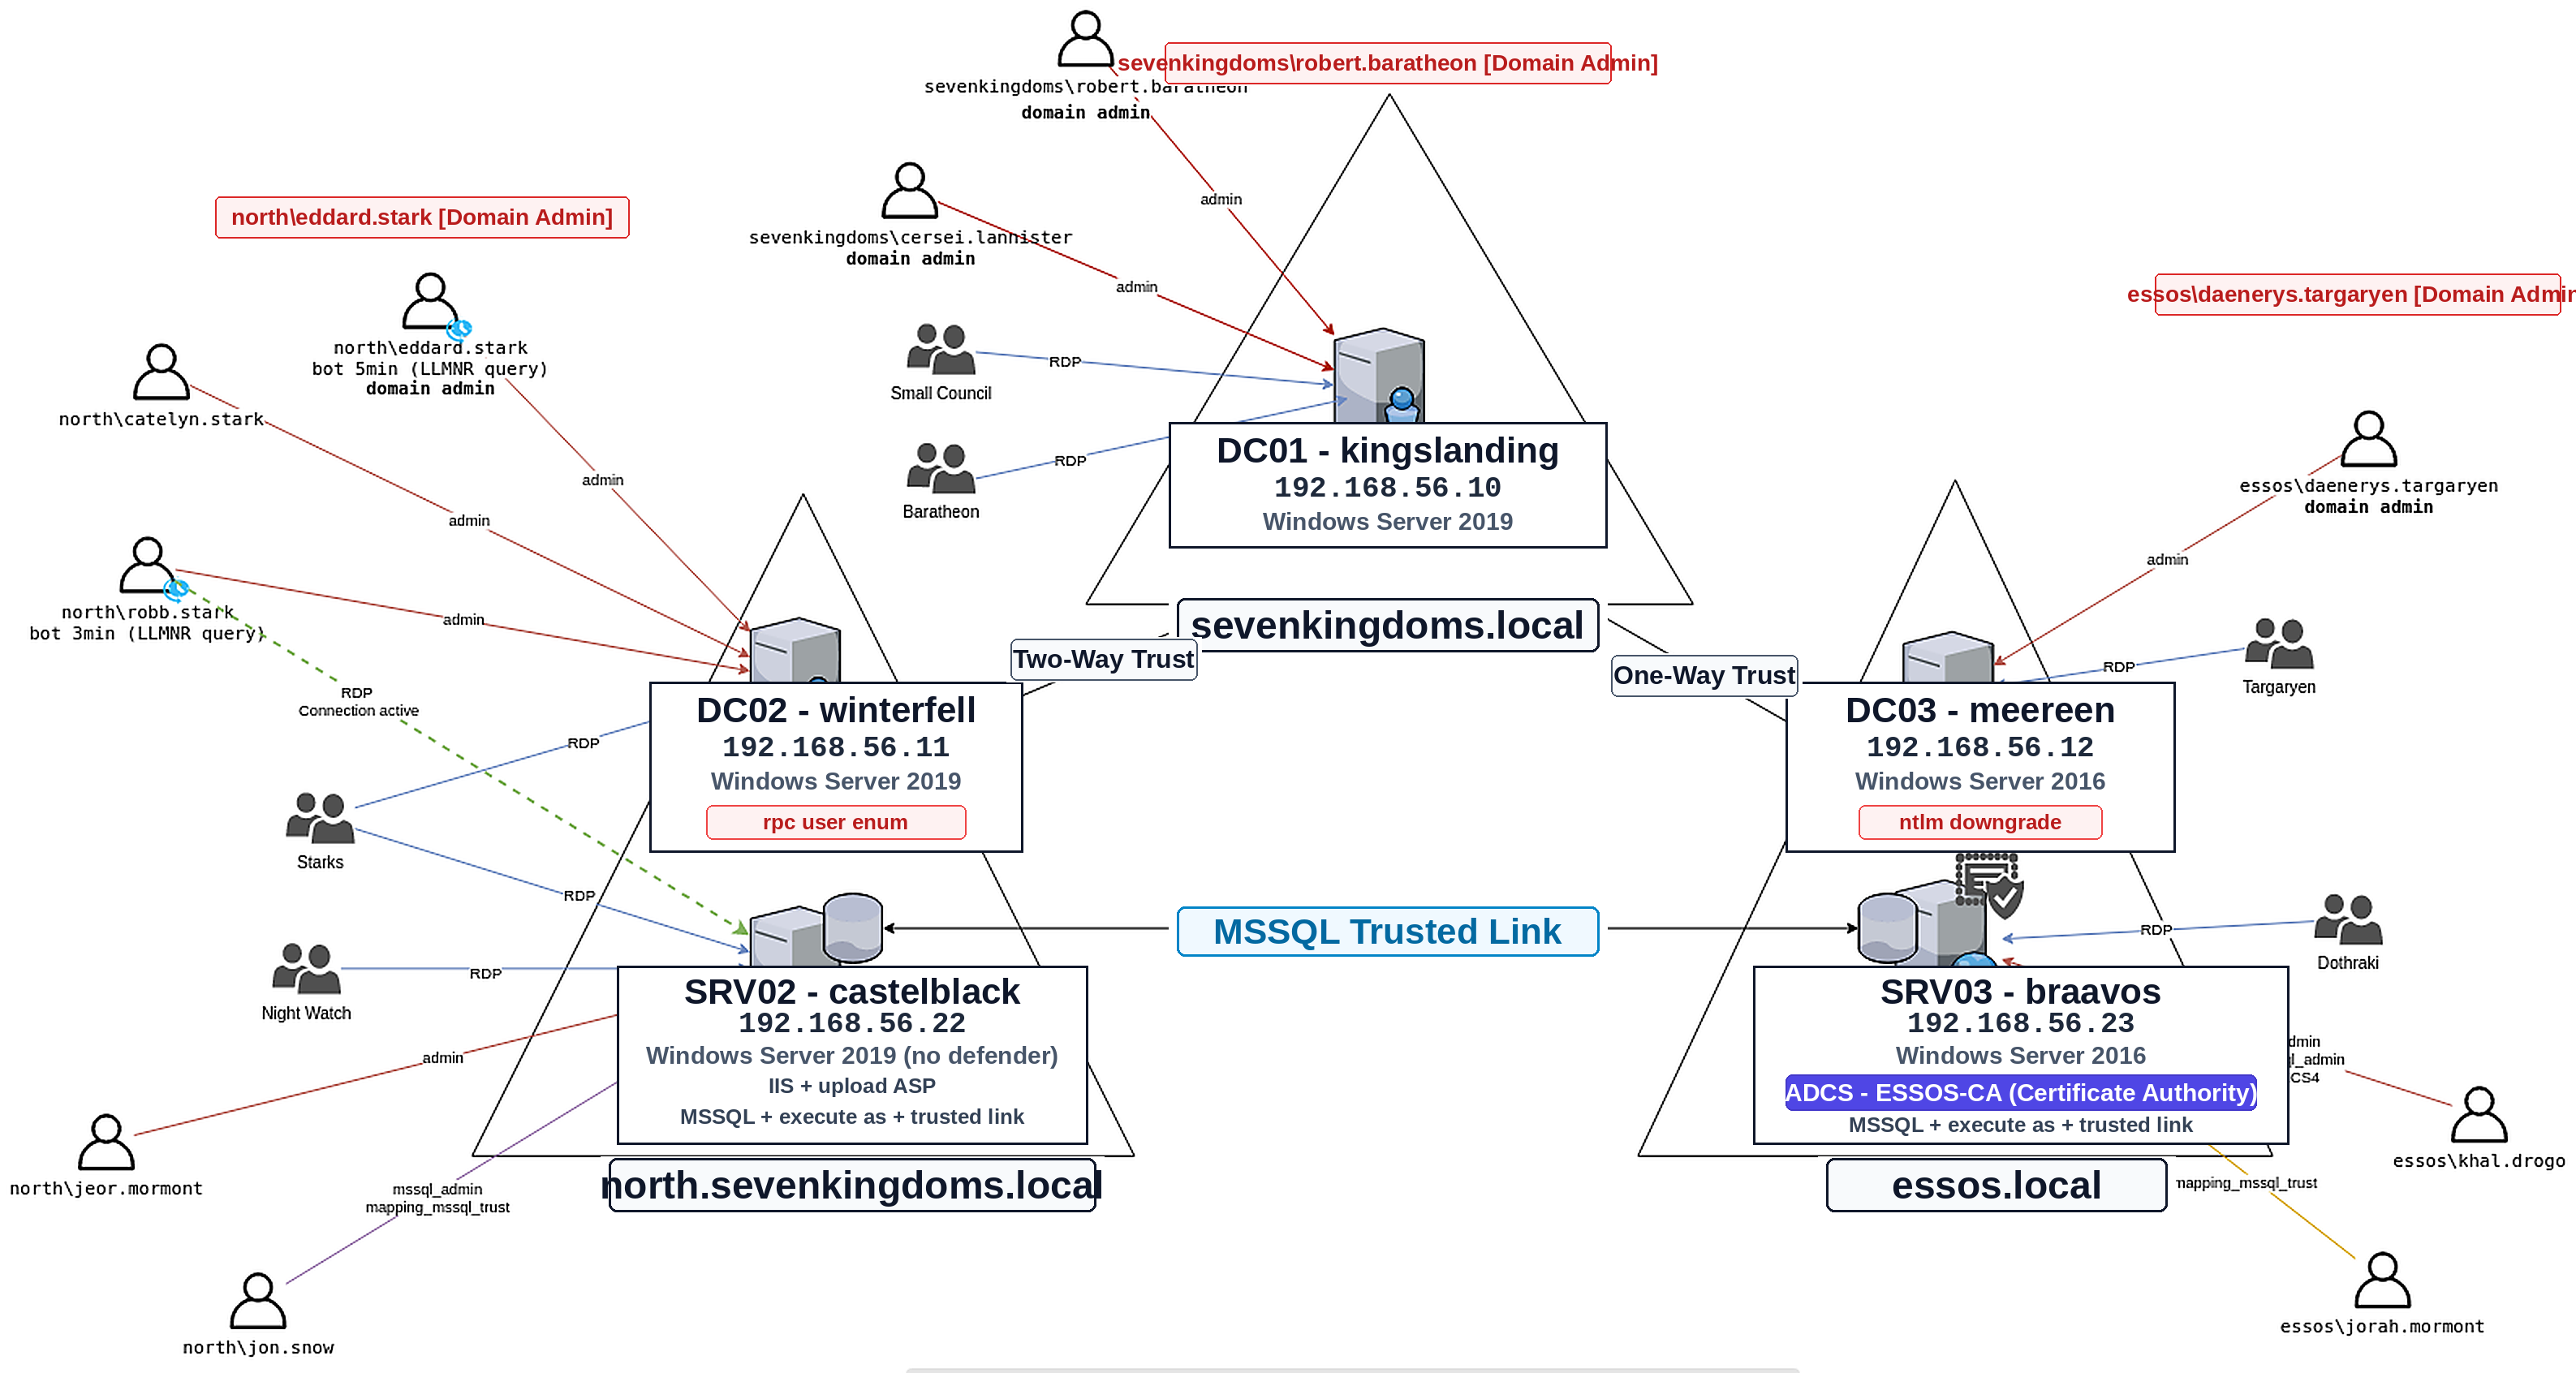
\includegraphics[width=\columnwidth]{figures/goad_forest_topology.png}
    \caption{Architecture and trust relationship schema of the Game of Active Directory (GOAD) enterprise testing environment.}
    \label{fig:goad_topology}
\end{figure}

CertGraph ingested 1,248 directory entities and 6,892 multi-relational edges via live LDAP collection. In zero-shot evaluation without fine-tuning, CertGraph successfully detected all 7 active privilege escalation vectors across both forests, including an ESC1 template published on \texttt{NORTH.sevenkingdoms.local} and an ESC13 issuance policy linkage on \texttt{BRAAVOS.essos.local}. The Two-Tier engine verified all attack paths within 145~ms, proving zero-shot domain transferability to authentic enterprise networks.

\section{Discussion, Limitations, and Conclusion}

\subsection{Limitations and Future Horizons}
While CertGraph achieves state-of-the-art performance, we acknowledge three scientific limitations:
\begin{enumerate}
    \item \textbf{Single-Label Formulation:} Currently, templates exhibiting multiple simultaneous vulnerabilities are assigned their highest-severity class. Future work will extend the classification head to multi-label sigmoid scoring.
    \item \textbf{Runtime Protocol Evasion:} CertGraph analyzes static directory permissions. Dynamic runtime coercion attacks (e.g., PetitPotam relay over HTTP) require integration with host event logging (ETW).
    \item \textbf{Cloud-Hybrid Identity Fabrics:} Modern enterprises increasingly synchronize on-premises Active Directory with Microsoft Entra ID (Azure AD). Extending the metagraph schema to model cloud-native OAuth permissions represents an important frontier.
\end{enumerate}

\subsection{Conclusion}
This paper presented CertGraph, a unified graph AI and neuro-symbolic verification framework for Active Directory Certificate Services. We proved that parameterized residual skip-connections are mathematically necessary to maintain gradient lower bounds across deep identity delegation chains (Theorem~1). Across 700 enterprise topologies, CertGraph achieved a 99.86\% Macro-F1. By discovering the phenomenon of neural shortcut collapse on adversarial hard negatives, we formulated a Two-Tier Neuro-Symbolic Engine that combines 18~ms neural screening with 110~ms symbolic verification to achieve zero false negatives and zero false alarms (128.8~ms total latency). Finally, we proved the NP-hardness of access interdiction (Theorem~2) and demonstrated autonomous, disruption-bounded remediation severing 68.6\% of attack paths, providing enterprise defenders with scalable, provable identity security.

\balance
\bibliographystyle{IEEEtran}
\bibliography{references}

\end{document}
